% =====================================================================
% ÉTAT DE L'ART
% =====================================================================
\chapter{État de l'Art}
\section{État de l'Art}
\label{sec:etat-art}

Le chapitre précédent a mis en lumière les défis structurels de la migration de données et formulé la problématique centrale de ce travail. Le présent chapitre explore l'état de l'art scientifique et technologique afin d'identifier les fondements, les solutions existantes, et les opportunités d'amélioration qui positionnent notre contribution. Nous commençons par les fondements théoriques, passons en revue les solutions du marché, décrivons en profondeur la plateforme ADMP dans son état actuel, explorons les avancées de l'intelligence artificielle appliquées au domaine, avant d'analyser les limites de l'existant et de formuler notre positionnement.

% =====================================================================
\subsection{Fondements théoriques}
\label{subsec:fondements}

% ---------------------------------------------------------------------
\subsubsection{Le paradigme ETL / ELT : principes et évolution}
\label{subsubsec:etl-elt}

Le paradigme \textbf{ETL (Extract, Transform, Load)} constitue depuis plusieurs décennies le socle fondamental de toute opération d'intégration de données. Il décrit un processus en trois phases séquentielles : l'\textbf{extraction} des données depuis les systèmes sources, leur \textbf{transformation} dans une zone intermédiaire (staging) pour les adapter au modèle cible, puis leur \textbf{chargement} dans le système de destination. Ce paradigme a été le pilier de l'ère du data warehousing classique, où les ressources de calcul étaient limitées et coûteuses, imposant un pré-traitement rigoureux des données avant leur insertion dans l'entrepôt.

Avec l'avènement du cloud computing et des entrepôts de données modernes (Snowflake, BigQuery, Amazon Redshift), un paradigme alternatif a émergé : l'\textbf{ELT (Extract, Load, Transform)}. Dans cette approche, les données brutes sont d'abord chargées dans le système cible, puis transformées directement en exploitant la puissance de calcul élastique de l'infrastructure cloud. L'ELT offre une flexibilité analytique accrue, une meilleure utilisation des ressources et un time-to-insight réduit, tout en posant de nouveaux défis en matière de gouvernance et de gestion technique.

\begin{figure}[H]
    \centering
    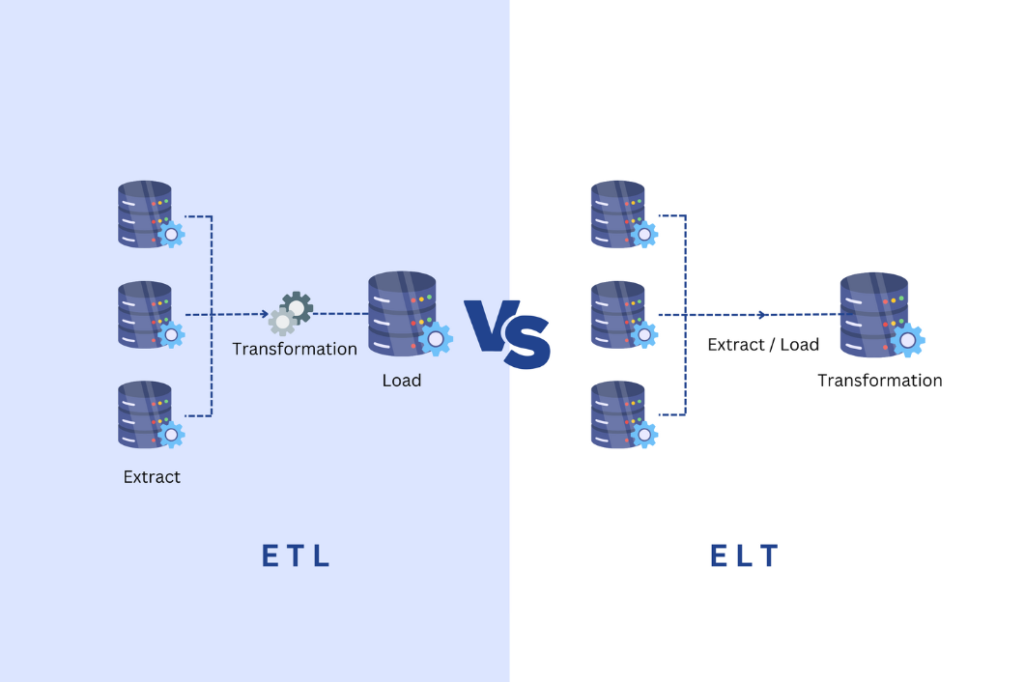
\includegraphics[width=0.9\textwidth]{img/ETL_VS_ELT.png}
    \caption{Comparaison des paradigmes ETL et ELT}
    \label{fig:etl-vs-elt}
\end{figure}

L'évolution de l'ETL vers l'ELT ne se résume pas à une simple réorganisation des étapes : elle reflète un changement fondamental dans la philosophie de gestion des données. Comme le souligne Vanga (2024) dans son étude publiée dans l'\textit{International Journal for Multidisciplinary Research}, cette transition est catalysée par la croissance exponentielle des volumes de données, la prolifération des sources hétérogènes, et les exigences d'analyse en temps réel. Les architectures modernes tendent vers des modèles hybrides combinant les forces des deux approches, avec l'émergence de concepts tels que le \textbf{zero-ETL} et le \textbf{data mesh} qui promettent de réduire encore la complexité des pipelines de données.
Le Tableau~\ref{tab:etl-elt-comparison} présente une comparaison synthétique des deux paradigmes.

\begin{table}[H]
\centering

\begin{tabularx}{\textwidth}{lXX}
\toprule
\textbf{Critère} & \textbf{ETL} & \textbf{ELT} \\
\midrule
Transformation & Avant le chargement (staging) & Après le chargement (in-warehouse) \\
\addlinespace
Infrastructure & On-premise, ressources limitées & Cloud-native, calcul élastique \\
\addlinespace
Flexibilité & Schéma rigide, pré-défini & Schéma flexible, late-binding \\
\addlinespace
Vitesse & Plus lent sur grands volumes & Plus rapide (puissance cloud) \\
\addlinespace
Gouvernance & Contrôle pré-chargement & Nécessite gouvernance SQL forte \\
\addlinespace
Outils typiques & Informatica, Talend, SSIS & dbt, Snowflake, BigQuery \\
\bottomrule
\end{tabularx}
\caption{Comparaison entre ETL et ELT}
\label{tab:etl-elt-comparison}
\end{table}

% ---------------------------------------------------------------------
\subsubsection{Modélisation des données}
\label{subsubsec:modelisation}

La réussite d'un projet de migration repose en grande partie sur la maîtrise des modèles de données source et cible. Trois approches principales de modélisation coexistent dans l'écosystème :

\begin{itemize}[leftmargin=*]
    \item \textbf{Le modèle relationnel}, fondé sur les travaux de Codd (1970), organise les données en tables liées par des clés primaires et étrangères. Il reste le standard dominant dans les systèmes transactionnels (OLTP) et les plateformes CRM comme Salesforce.
    
    \item \textbf{Le modèle dimensionnel}, popularisé par Kimball, structure les données autour de tables de faits et de dimensions, optimisées pour l'analyse (OLAP). Il est au cœur des entrepôts de données classiques.
    
    \item \textbf{Le modèle orienté objet}, qui encapsule données et comportements dans des objets liés par héritage et composition, est utilisé dans les systèmes modernes et les plateformes cloud-native. Comme le détaille la formation CIDS d'ADMP, \og~\textit{an object-oriented data model consists of basic concepts: Object, Object identifier, Attributes, Methods, Class, Class hierarchy, and Inheritance}~\fg{}.
\end{itemize}

La compréhension de ces modèles est essentielle pour le Data Analyst qui doit établir les correspondances (mappings) entre le système source et le système cible, en tenant compte des différences structurelles, des contraintes d'intégrité et des relations entre entités.

% ---------------------------------------------------------------------
\subsubsection{Qualité des données : métriques et frameworks}
\label{subsubsec:qualite-donnees}

La qualité des données est un facteur déterminant du succès de toute migration. Le concept de dimensions de qualité des données a été formalisé en 1996 par les professeurs Richard Y. Wang et Diane M. Strong dans leur article fondateur \og~\textit{Beyond Accuracy: What Data Quality Means to Data Consumers}~\fg{}. Depuis, le framework DAMA-DMBOK a standardisé \textbf{six dimensions fondamentales} universellement adoptées, présentées dans le Tableau~\ref{tab:data-quality}.

\begin{table}[H]
\centering

\begin{tabularx}{\textwidth}{lXX}
\toprule
\textbf{Dimension} & \textbf{Description} & \textbf{Exemple d'impact en migration} \\
\midrule
Exactitude & Les données reflètent-elles fidèlement la réalité ? & Adresse client erronée → livraison échouée \\
\addlinespace
Complétude & Tous les champs requis sont-ils renseignés ? & Champ obligatoire vide → rejet au chargement \\
\addlinespace
Cohérence & Les données sont-elles uniformes entre systèmes ? & Prix différent entre web et mobile \\
\addlinespace
Fraîcheur & Les données sont-elles disponibles à temps ? & Données obsolètes → décisions erronées \\
\addlinespace
Validité & Les données respectent-elles les formats et règles ? & Date \og~30 février~\fg{} → rejet de validation \\
\addlinespace
Unicité & Pas de doublons ? & Doublons clients → métriques faussées \\
\bottomrule
\end{tabularx}
\caption{Dimensions de la qualité des données et impact en migration}
\label{tab:data-quality}
\end{table}

Le coût de la non-qualité est considérable : selon Gartner (2023), la mauvaise qualité des données coûte en moyenne \textbf{12,9 millions de dollars par an} aux organisations. Dans le contexte spécifique de la migration, la mise en place de contrôles de qualité automatisés (profiling, validation pré-chargement, réconciliation post-chargement) est donc un prérequis incontournable.

\begin{figure}[H]
    \centering
    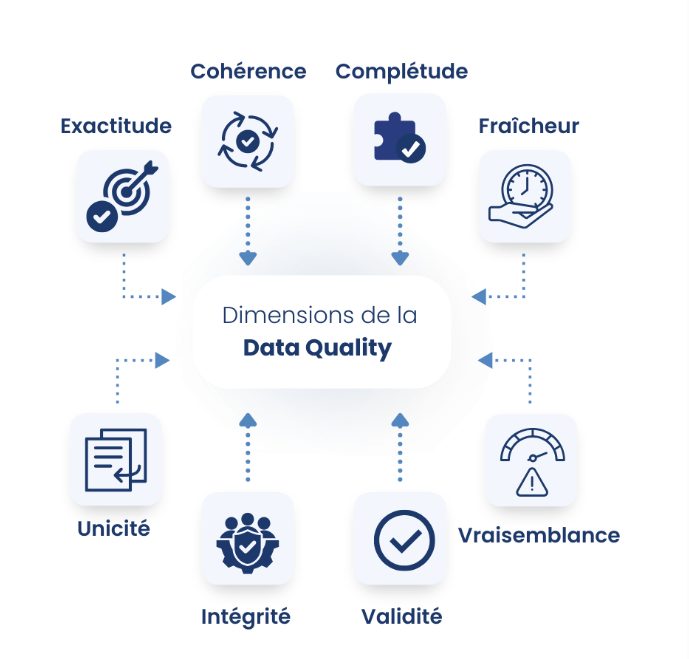
\includegraphics[width=0.7\textwidth]{img/Qualité de data.png}
    \caption{Les dimensions de la qualité des données }
    \label{fig:data-quality}
\end{figure}

% ---------------------------------------------------------------------
\subsubsection{Gouvernance des données et conformité}
\label{subsubsec:gouvernance}

La gouvernance des données établit les politiques, processus et responsabilités qui encadrent la gestion des données tout au long de leur cycle de vie. Dans le contexte de la migration, elle revêt une importance critique pour trois raisons :

Premièrement, la \textbf{traçabilité des données} (\textit{data lineage}), la capacité à retracer le parcours complet d'une donnée depuis son origine jusqu'à sa destination, en passant par chaque transformation, est devenue une exigence réglementaire explicite. Le RGPD (Article 30) impose aux organisations de maintenir des registres des activités de traitement, incluant la classification des données, le suivi de la qualité, et les politiques de rétention.

Deuxièmement, le \textbf{principe de responsabilité} (\textit{accountability}, Article 5(2) du RGPD) exige que les organisations puissent \textbf{démontrer}, et non simplement affirmer, leur conformité, à travers des politiques documentées, des rôles définis, des contrôles techniques et des traces d'audit.

Troisièmement, les réglementations émergentes comme l'\textbf{EU AI Act} ajoutent une couche supplémentaire de complexité : les organisations utilisant l'IA dans leurs processus de migration doivent documenter de manière exhaustive les flux de données, avec des amendes pouvant atteindre \textbf{7,5 à 35 millions d'euros} en cas de non-conformité.

L'intégration du data lineage dans le cadre de gouvernance offre des avantages concrets : amélioration de la redevabilité, support au troubleshooting, analyse d'impact proactive lors des mises à jour, et simplification des audits de conformité.

\begin{figure}[H]
    \centering
    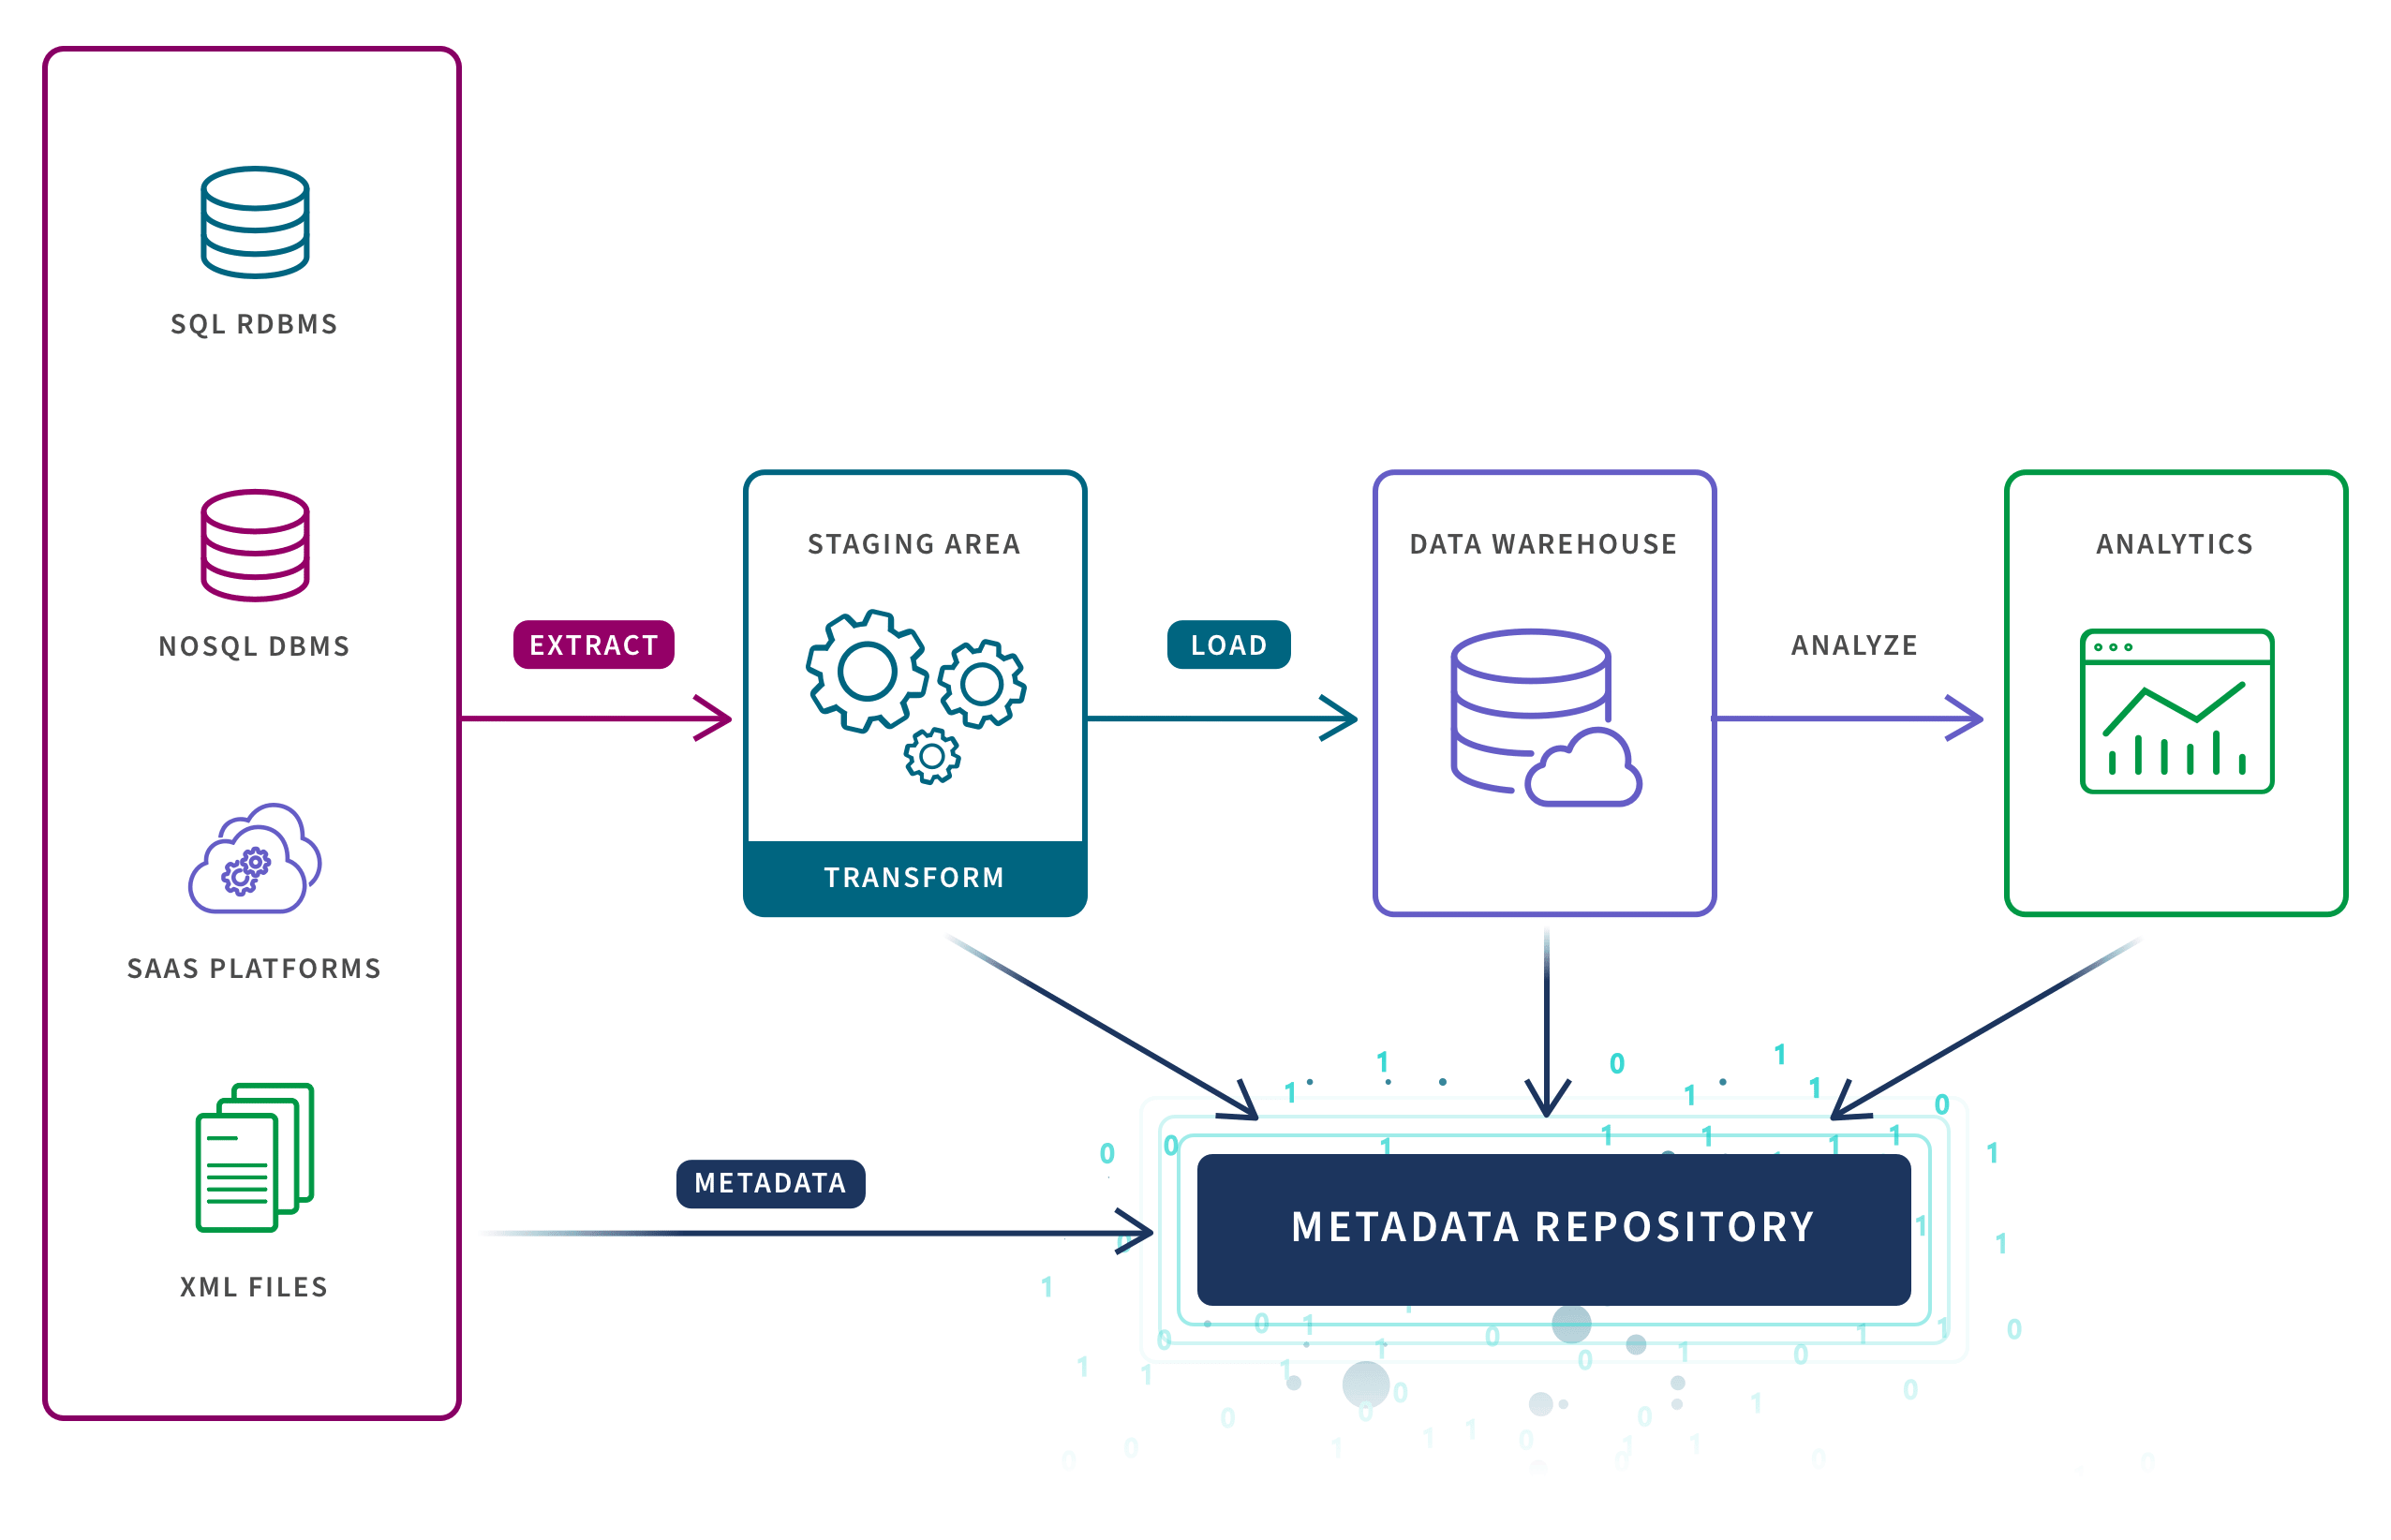
\includegraphics[width=0.85\textwidth]{img/data_lineage.png}
    \caption{Exemple de traçabilité des données (Data Lineage)}
    \label{fig:data-lineage}
\end{figure}

% =====================================================================
\subsection{Solutions existantes sur le marché}
\label{subsec:solutions-marche}

% ---------------------------------------------------------------------
\subsubsection{Outils ETL traditionnels}
\label{subsubsec:etl-traditionnels}

Le marché des outils ETL traditionnels est dominé par trois acteurs majeurs, chacun avec ses forces et ses limites :

\textbf{Informatica PowerCenter} est considéré comme la référence enterprise-grade. Il offre une large connectivité (Oracle, DB2, Teradata, NoSQL), un profilage automatique des données, et des mécanismes robustes de gestion des erreurs. Cependant, son coût de licence élevé, sa courbe d'apprentissage abrupte et son interface vieillissante limitent son accessibilité.

\textbf{Talend} propose une approche open-source (Talend Open Studio) complétée par une édition enterprise. Basé sur Java, il offre plus de 900 connecteurs, un support natif du Big Data (Hadoop, Spark), et une interface drag-and-drop accessible. Il constitue un choix privilégié pour les organisations cherchant flexibilité et maîtrise des coûts.

\textbf{SSIS (SQL Server Integration Services)} de Microsoft est intégré à SQL Server sans coût de licence additionnel. Performant dans les environnements Microsoft-centric, il souffre néanmoins d'un support limité pour les systèmes non-Microsoft et d'une scalabilité restreinte en environnements hétérogènes.

Le Tableau~\ref{tab:etl-tools-comparison} présente une comparaison détaillée de ces trois outils.

\begin{table}[H]
\centering
\caption{Comparaison des outils ETL traditionnels}
\label{tab:etl-tools-comparison}
\begin{tabularx}{\textwidth}{lXXX}
\toprule
\textbf{Critère} & \textbf{Informatica} & \textbf{Talend} & \textbf{SSIS} \\
\midrule
Type & Propriétaire & Open-source + Enterprise & Propriétaire (inclus SQL Server) \\
\addlinespace
Coût & Élevé & Gratuit (OS) / Modéré (Ent.) & Inclus avec SQL Server \\
\addlinespace
Cloud & Fort (IICS) & Excellent (cloud-native) & Limité (via ADF) \\
\addlinespace
Big Data & Add-ons requis & Support natif (Spark, Hadoop) & Support basique \\
\addlinespace
Connectivité & Très large & 900+ connecteurs & Fort en Microsoft \\
\addlinespace
Courbe d'apprentissage & Raide & Modérée & Modérée \\
\bottomrule
\end{tabularx}
\end{table}

% ---------------------------------------------------------------------
\subsubsection{Services cloud natifs}
\label{subsubsec:cloud-natifs}

L'essor du cloud a donné naissance à des services d'intégration de données entièrement managés :

\textbf{AWS Glue} est un service ETL serverless basé sur Apache Spark, intégré à l'écosystème AWS (S3, Redshift, Athena). Il propose un Data Catalog automatisé, le support batch et streaming, et un studio visuel de développement de pipelines.

\textbf{Azure Data Factory (ADF)} de Microsoft offre plus de 90 connecteurs natifs, des Data Flows Spark pour les transformations no-code, et un runtime d'intégration hybride permettant de connecter données on-premise et cloud. Son intégration avec Azure Synapse, Databricks et Power BI en fait un choix naturel pour les organisations dans l'écosystème Microsoft.

\textbf{Google Cloud Dataflow}, basé sur Apache Beam, se distingue par son modèle unifié batch/streaming et sa facturation à la seconde. Il excelle dans le traitement en temps réel et les workloads analytiques avancés.

Le Tableau~\ref{tab:cloud-services-comparison} compare ces trois services cloud.

\begin{table}[H]
\centering
\caption{Comparaison des services cloud natifs}
\label{tab:cloud-services-comparison}
\begin{tabularx}{\textwidth}{lXXX}
\toprule
\textbf{Critère} & \textbf{AWS Glue} & \textbf{Azure Data Factory} & \textbf{GCP Dataflow} \\
\midrule
Moteur & Apache Spark & Spark (Data Flows) & Apache Beam \\
\addlinespace
Modèle & Serverless & Serverless + IR & Serverless \\
\addlinespace
Connecteurs & 70+ & 90+ & Google Cloud natif \\
\addlinespace
Streaming & Oui (Kinesis, MSK) & Limité & Excellent (Pub/Sub) \\
\addlinespace
Coût/TB batch & $\sim$1,84 & $\sim$1,42 & $\sim$2,11 \\
\addlinespace
Latence streaming p99 & $\sim$120ms & $\sim$148ms & $\sim$89ms \\
\bottomrule
\end{tabularx}
\end{table}

% ---------------------------------------------------------------------
\subsubsection{Approches ad hoc / scripts custom}
\label{subsubsec:scripts-custom}

De nombreuses organisations développent encore des scripts ad hoc (SQL, Python, Shell) pour gérer leurs migrations. Cette approche offre une flexibilité maximale et un coût initial faible, mais présente des limites critiques : absence de standardisation, aucune traçabilité intrinsèque, dépendance aux développeurs individuels, maintenance difficile, et risque élevé d'erreurs sur les projets à grande échelle.

% ---------------------------------------------------------------------
\subsubsection{Analyse comparative et limites communes}
\label{subsubsec:limites-communes}

Malgré leurs différences, toutes ces solutions partagent des limitations structurelles communes :

\begin{itemize}[leftmargin=*]
    \item \textbf{Le fossé Design-Build} : dans chaque cas, les spécifications fonctionnelles doivent être traduites manuellement en code exécutable par une équipe technique, créant un risque permanent de décalage entre le design et l'implémentation.
    
    \item \textbf{Effet boîte noire} : les moteurs ETL traditionnels ne permettent pas aux équipes fonctionnelles de vérifier directement que le code implémenté correspond aux spécifications validées.
    
    \item \textbf{Absence de couche métier} : les services cloud natifs sont performants pour le transport de données, mais manquent de la couche fonctionnelle nécessaire pour gérer les règles de transformation complexes, les Key Decisions, et la validation métier itérative.
    
    \item \textbf{Coûts cachés} : licences logicielles, infrastructure dédiée, main-d'œuvre technique spécialisée, et coûts de maintenance s'accumulent au fil du projet.
\end{itemize}

C'est dans ce contexte que la plateforme ADMP se positionne comme une réponse industrielle visant à combler ces lacunes.

% =====================================================================
\subsection{La plateforme ADMP : état actuel}
\label{subsec:admp-actuel}

% ---------------------------------------------------------------------
\subsubsection{Envergure mondiale et chiffres clés}
\label{subsubsec:admp-envergure}

\begin{figure}[H]
    \centering
    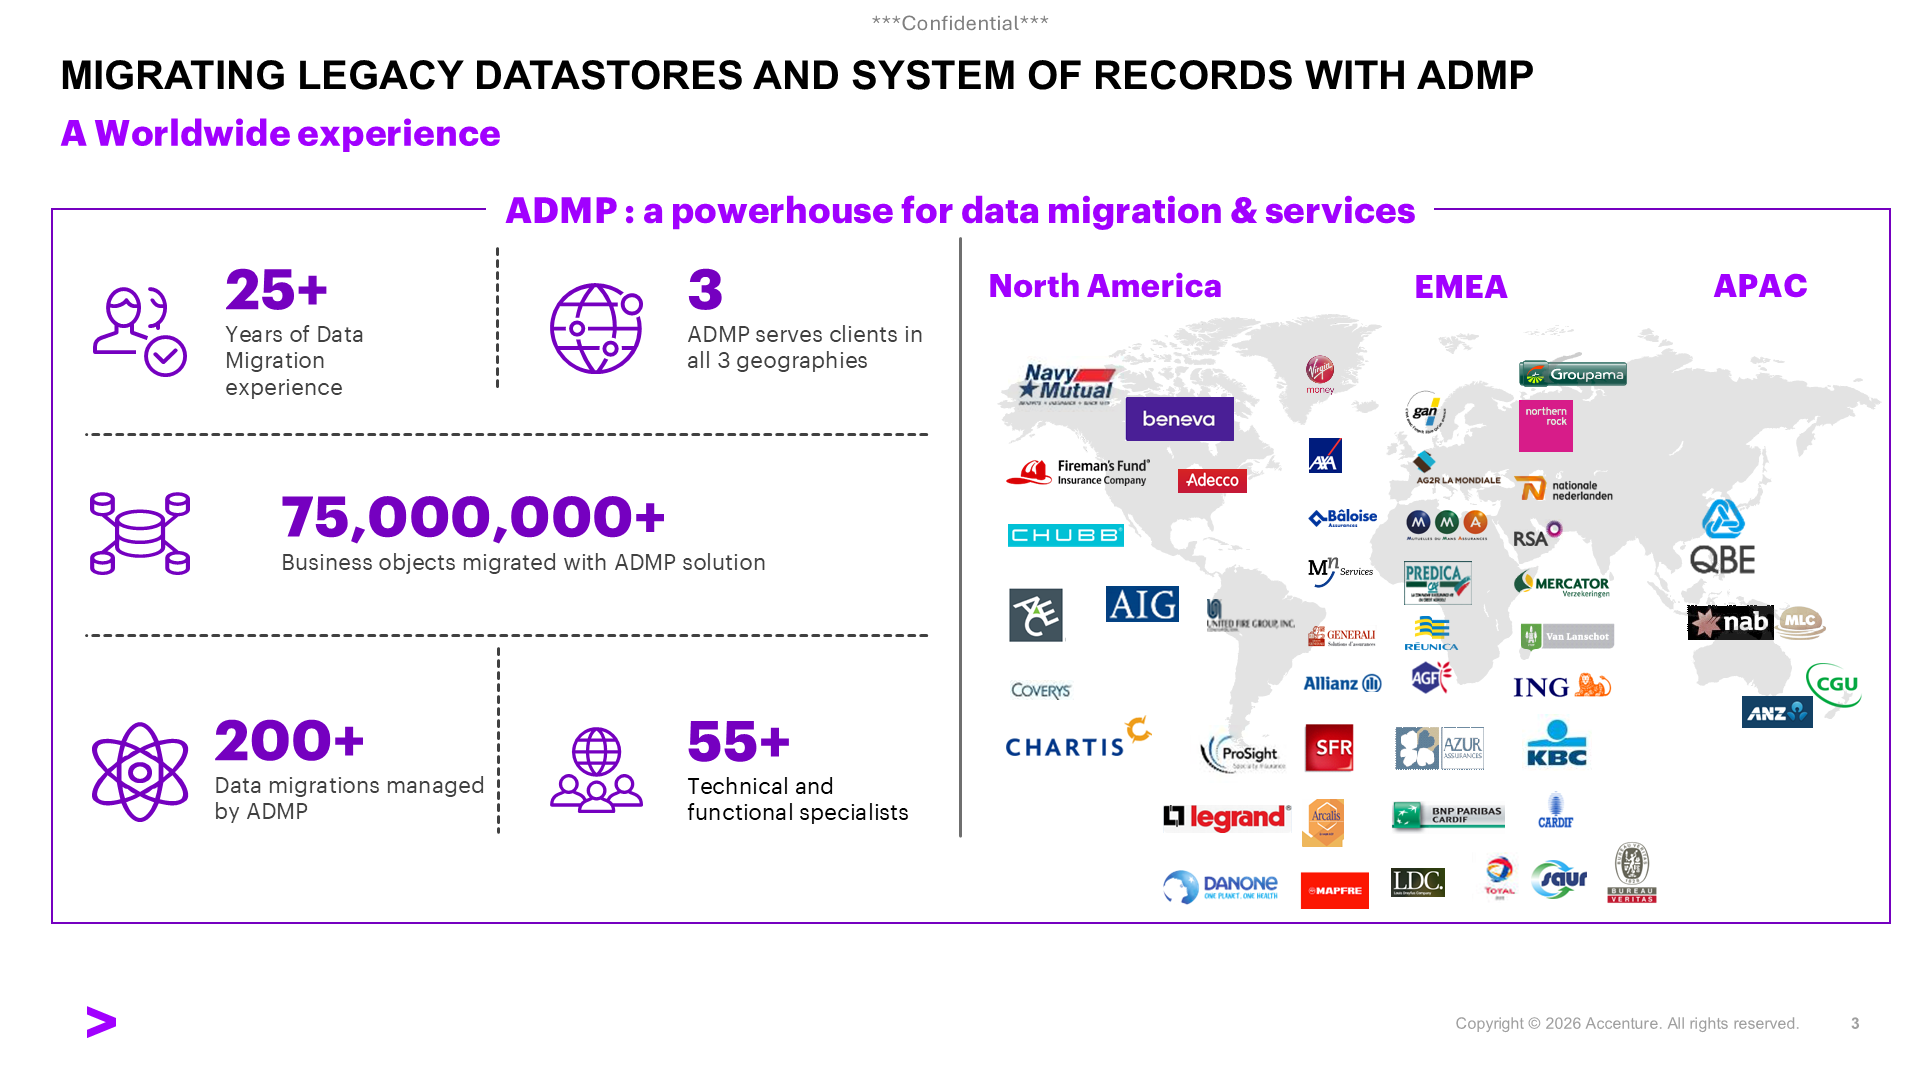
\includegraphics[width=0.85\textwidth]{img/admp_worldwide.png}
    \caption{Envergure mondiale de la plateforme ADMP : chiffres clés et 3 géographies}
    \label{fig:admp-worldwide}
\end{figure}

L'\textbf{Accenture Data Migration Platform (ADMP)} est une solution propriétaire d'Accenture dédiée à la migration de données d'entreprise à grande échelle. Forte de plus de \textbf{25 ans d'expérience}, la plateforme a accompagné plus de \textbf{200 projets de migration} à travers le monde, avec plus de \textbf{75 millions d'objets métier migrés} par une équipe de plus de \textbf{55 spécialistes} techniques et fonctionnels. La plateforme intervient dans \textbf{3 géographies} : North America, APAC et EMEA, positionnant ADMP comme \og~\textit{a powerhouse for data migration \& services}~\fg{}.

% ---------------------------------------------------------------------
\subsubsection{Quatre piliers de valeur}
\label{subsubsec:admp-piliers}

\begin{figure}[H]
    \centering
    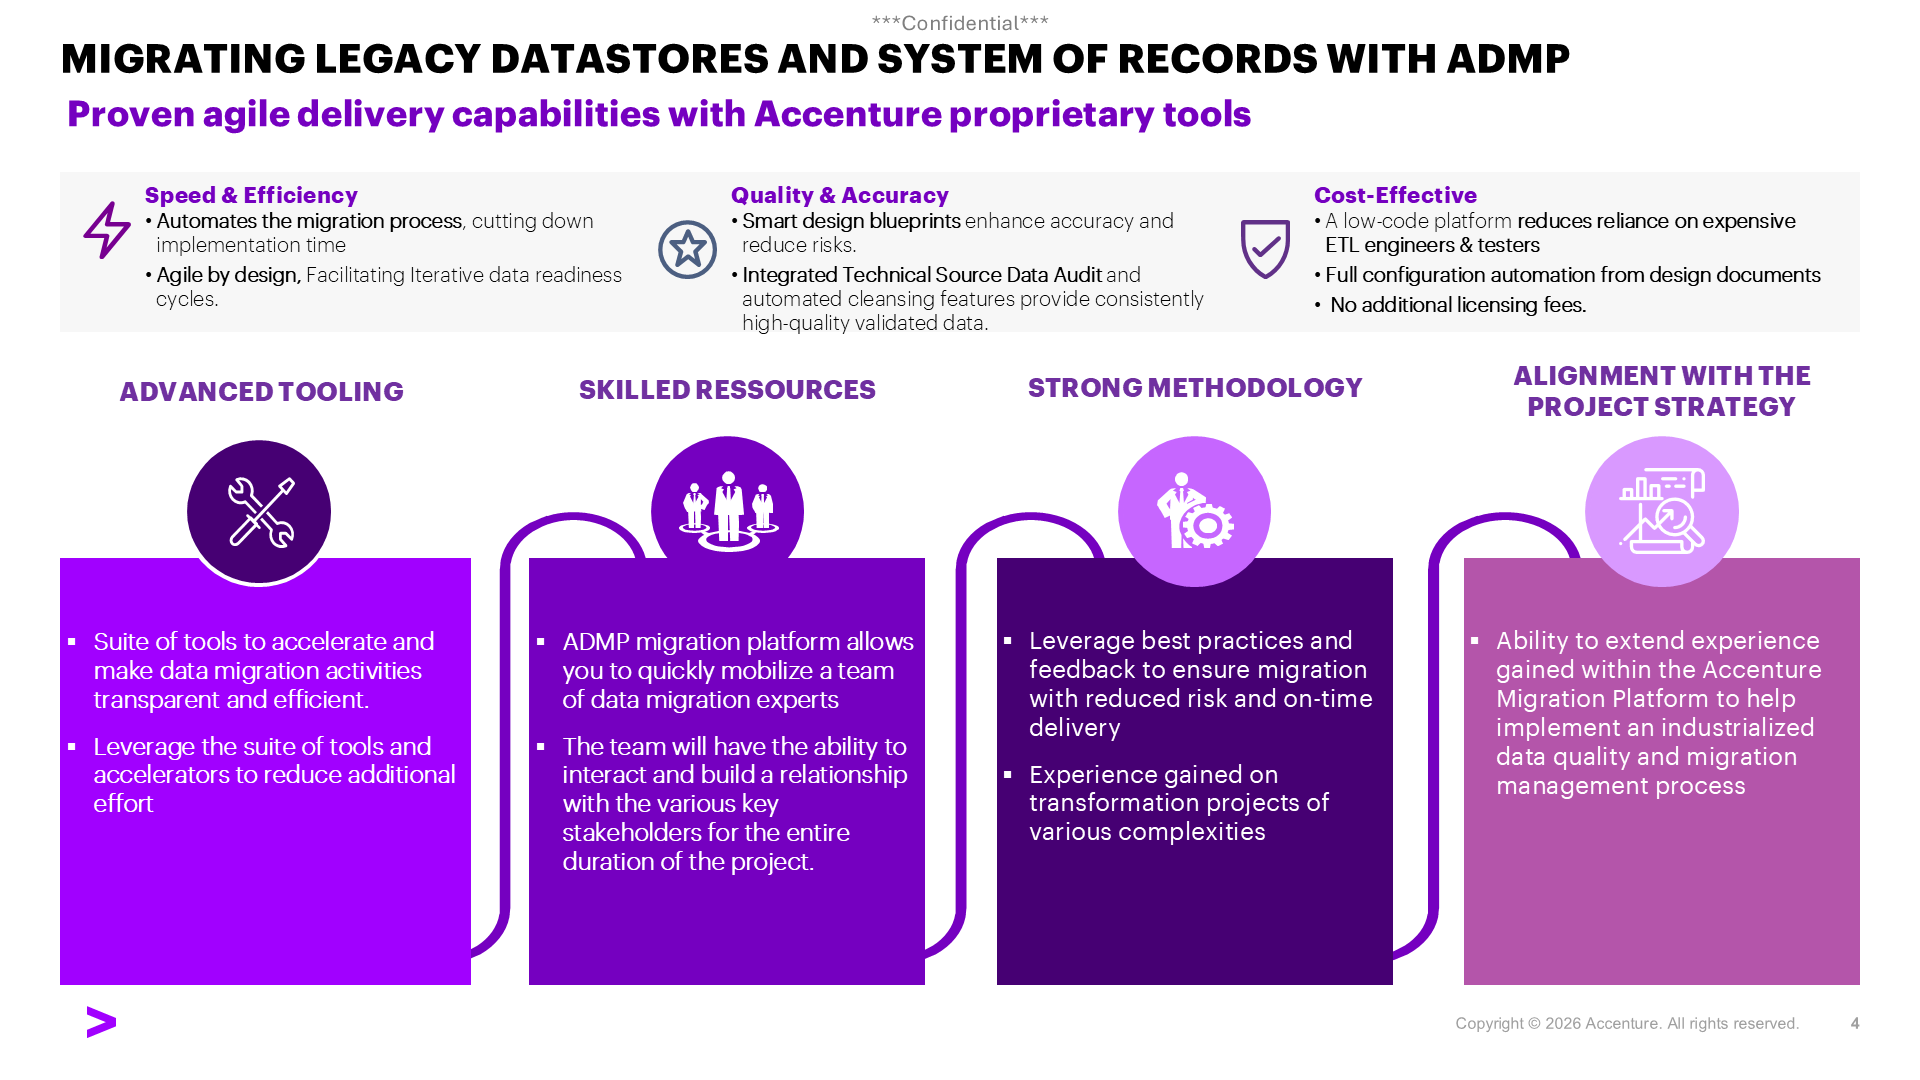
\includegraphics[width=0.85\textwidth]{img/admp_pillars.png}
    \caption{Les quatre piliers de valeur de la plateforme ADMP}
    \label{fig:admp-pillars}
\end{figure}

La valeur d'ADMP repose sur quatre piliers complémentaires qui structurent l'offre de service :

\begin{itemize}[leftmargin=*]
    \item \textbf{Advanced Tooling} : une suite d'outils et d'accélérateurs permettant de rendre les activités de migration transparentes et efficaces, et d'en réduire la charge additionnelle.
    \item \textbf{Skilled Resources} : la capacité à mobiliser rapidement une équipe d'experts en migration de données, capable d'interagir avec l'ensemble des parties prenantes tout au long du projet.
    \item \textbf{Strong Methodology} : un ensemble de meilleures pratiques éprouvées et validées, de la phase de découverte jusqu'au déploiement, garantissant une livraison dans les délais avec un risque réduit. \og~\textit{Experience gained on transformation projects of various complexities}~\fg{}.
    \item \textbf{Alignment with the Project Strategy} : la capacité à étendre l'expérience acquise sur la plateforme pour aider à mettre en \oe uvre un processus industrialisé de gestion de la qualité et de la migration des données.
\end{itemize}

% ---------------------------------------------------------------------
\subsubsection{Un service de migration sur mesure}
\label{subsubsec:admp-service}

\begin{figure}[H]
    \centering
    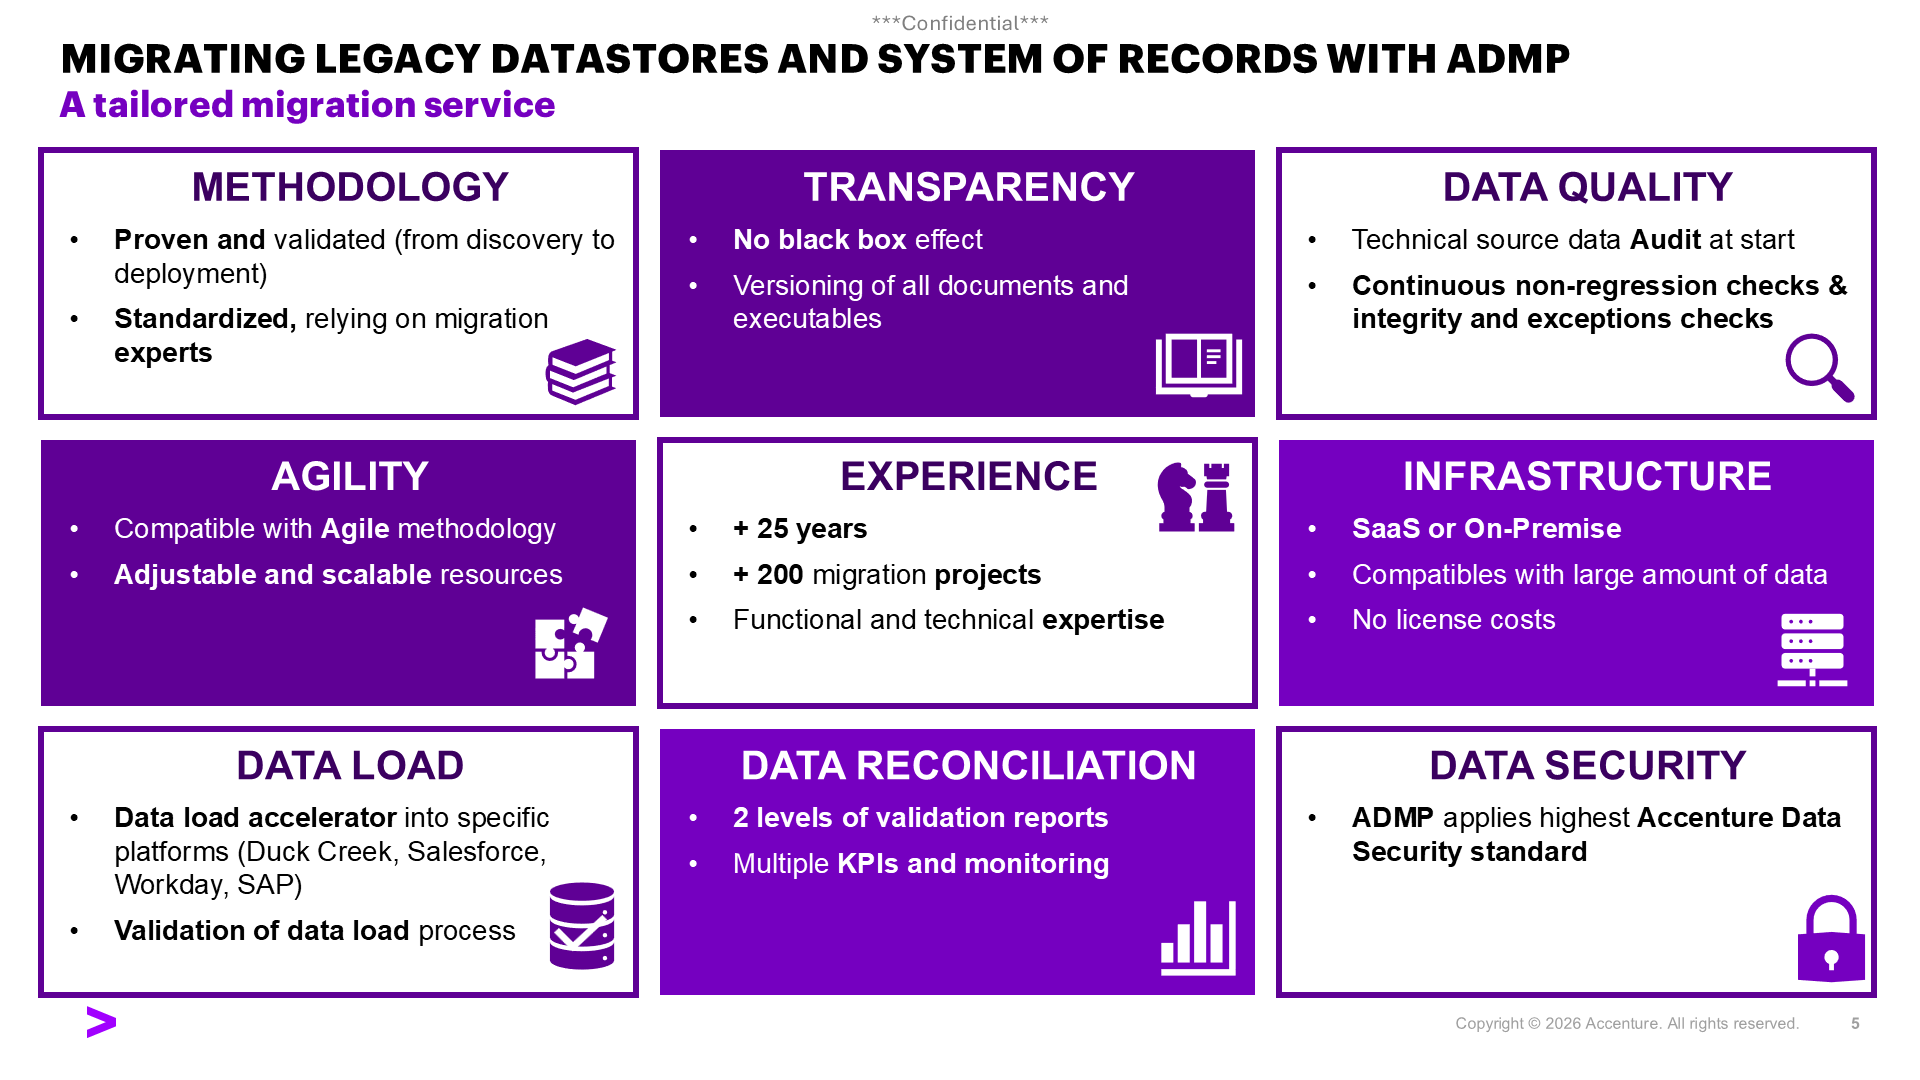
\includegraphics[width=0.85\textwidth]{img/admp_service_dimensions.png}
    \caption{Les neuf dimensions du service de migration sur mesure ADMP}
    \label{fig:admp-service}
\end{figure}

ADMP propose un service de migration global articulé autour de neuf dimensions clés :

\begin{itemize}[leftmargin=*]
    \item \textbf{Methodology} : méthodologie éprouvée et validée (de la découverte au déploiement), standardisée, s'appuyant sur des experts en migration.
    \item \textbf{Agility} : compatible avec les méthodes Agile, avec des ressources ajustables et scalables.
    \item \textbf{Data Load} : accélérateur de chargement vers des plateformes spécifiques (Duck Creek, Salesforce, Workday, SAP) avec validation du processus de chargement.
    \item \textbf{Transparency} : \og~\textit{No black box effect}~\fg{}, avec versioning de tous les documents et exécutables.
    \item \textbf{Experience} : +25 ans, +200 projets de migration, expertise fonctionnelle et technique.
    \item \textbf{Data Reconciliation} : 2 niveaux de rapports de validation, multiples KPIs et monitoring.
    \item \textbf{Data Quality} : audit technique des données source en amont, contrôles de non-régression continus, vérifications d'intégrité et gestion des exceptions.
    \item \textbf{Infrastructure} : SaaS ou On-Premise, compatible avec de grands volumes de données, sans coût de licence.
    \item \textbf{Data Security} : application des normes de sécurité des données les plus strictes d'Accenture.
\end{itemize}

% ---------------------------------------------------------------------
\subsubsection{Architecture end-to-end : le flux ETL ADMP}
\label{subsubsec:admp-etl}

\begin{figure}[H]
    \centering
    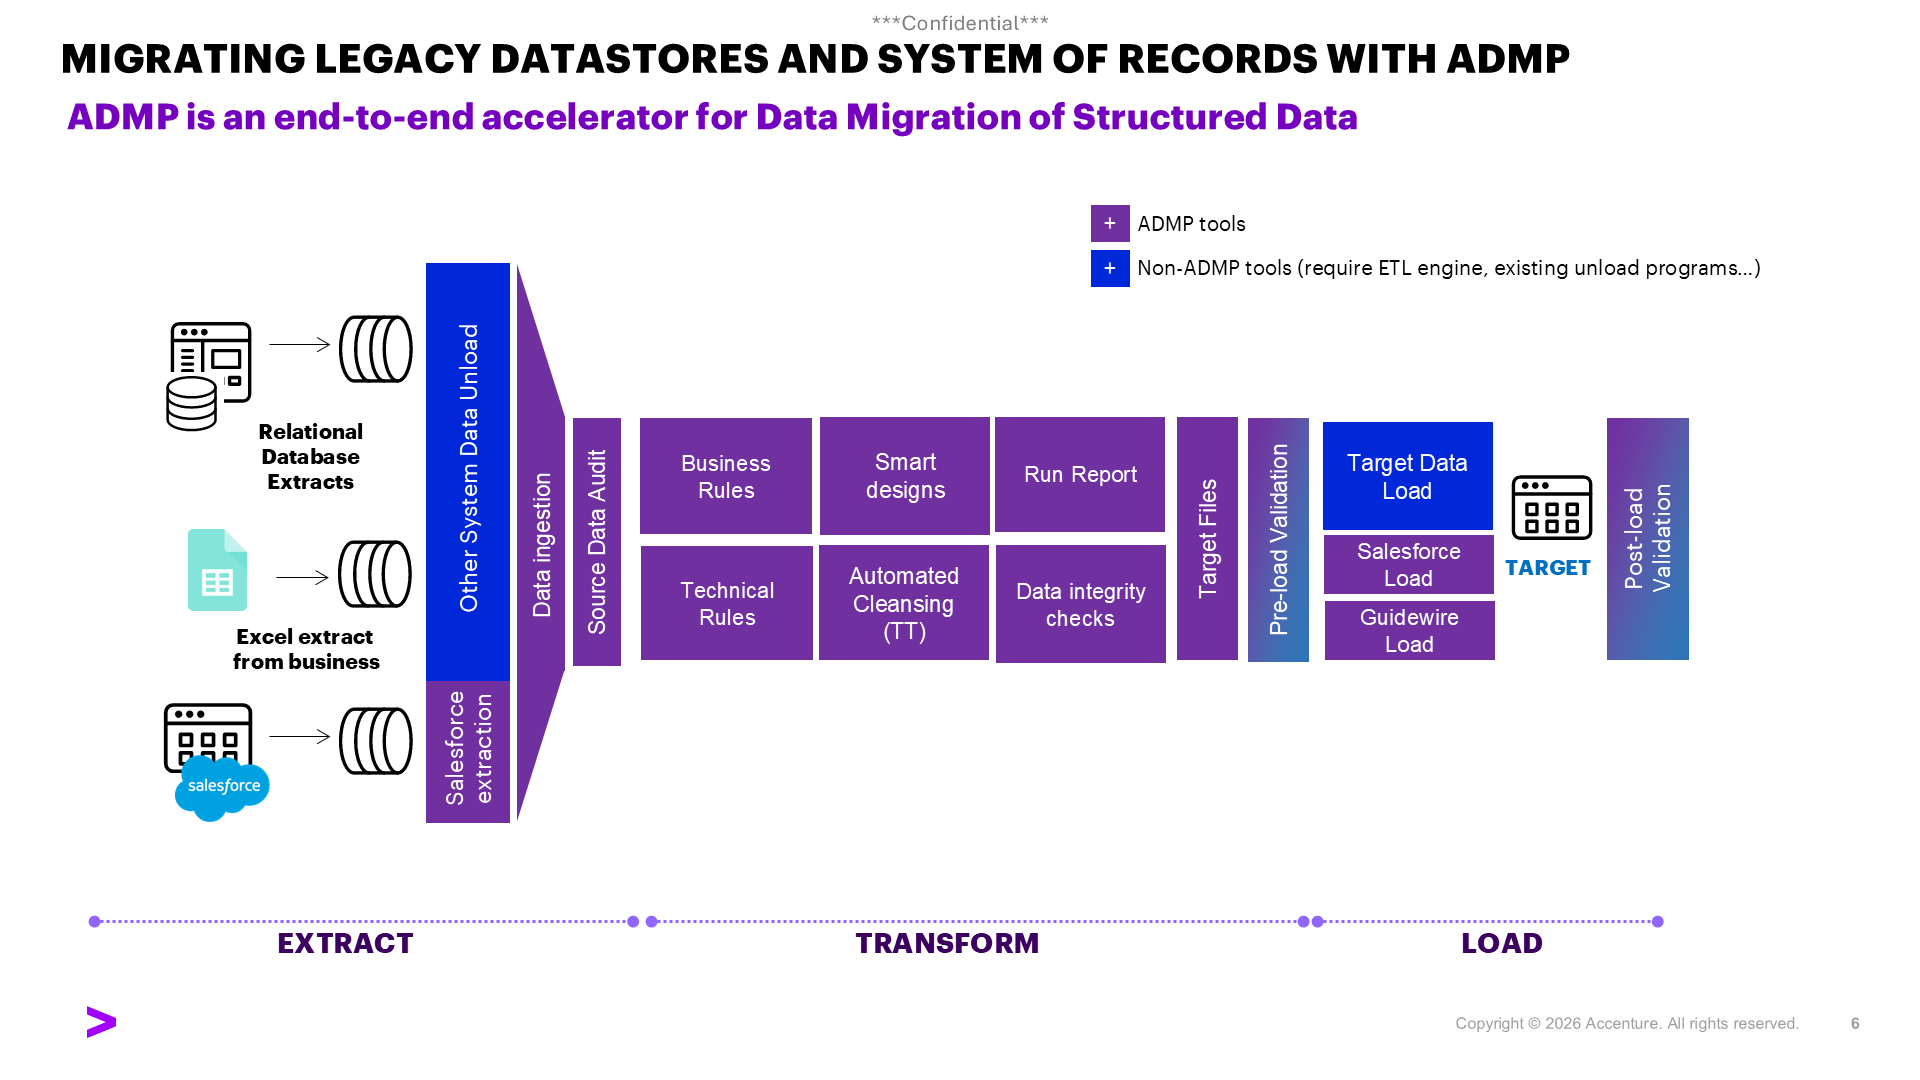
\includegraphics[width=\textwidth]{img/admp_etl_flow.png}
    \caption{Architecture end-to-end du flux ETL ADMP (Extract → Transform → Load)}
    \label{fig:admp-etl}
\end{figure}

Pour comprendre la valeur réelle d'ADMP, il convient de suivre le parcours d'une donnée depuis son système source jusqu'au système cible, en traversant chaque composant de la plateforme. Cette architecture, illustrée par la Figure~\ref{fig:admp-etl}, s'inscrit dans le modèle classique \textbf{Extract-Transform-Load (ETL)}, mais chaque phase est enrichie de composants propriétaires ADMP qui automatisent et sécurisent le processus. Il est important de noter que la plateforme distingue deux catégories de composants : les \textbf{outils ADMP} (développés et maîtrisés par Accenture) qui constituent le c\oe ur de la valeur ajoutée, et les \textbf{outils non-ADMP} (spécifiques aux systèmes source et cible du client) qui assurent les interfaces d'entrée et de sortie.

\paragraph{Phase 1 : Extract --- La collecte sécurisée des données sources.}

Le processus débute par l'extraction des données depuis les systèmes legacy du client. Ces données peuvent provenir de sources hétérogènes : bases de données relationnelles (Oracle, SQL Server, DB2, Mainframe), fichiers Excel fournis par les équipes métier, ou environnements Salesforce existants. À ce stade, les programmes d'\textit{unload} utilisés sont des outils \textbf{non-ADMP} : chaque système legacy dispose de son propre mécanisme d'export, que l'équipe adapte au contexte du projet.

Une fois extraits, les fichiers (généralement au format TXT ou CSV) sont pris en charge par le composant \textbf{Data Ingestion}, premier composant \textbf{ADMP} du pipeline. Celui-ci ingère les données dans la plateforme via un protocole de transfert sécurisé (SFTP, VPN), garantissant la confidentialité et l'intégrité des données dès leur entrée dans le périmètre Accenture.

\paragraph{Phase 2 : Transform --- Le c\oe ur de valeur d'ADMP.}

La phase de transformation est celle où ADMP déploie l'essentiel de son intelligence. Elle s'articule en deux couches fonctionnelles complémentaires.

La \textit{première couche} est dédiée à l'\textbf{audit et à la définition des règles}. Le composant \textbf{Source Data Audit} procède à un audit technique automatique et exhaustif de chaque table, enregistrement et champ source : il valide la complétude de l'extraction, détecte les anomalies de format et produit un état des lieux précis des données disponibles. C'est sur cette base que l'équipe de design commence son travail. Les \textbf{Business Rules} (règles métier fonctionnelles, correspondant aux documents RC --- \textit{Record Creation}) et les \textbf{Smart Designs} (l'ensemble des documents de spécification SDS, IDS, TDS, DS, DP, TT) constituent la \textit{source unique de vérité} du projet : le moteur ADMP lit ces documents et génère automatiquement les programmes de transformation, sans aucun développement ETL manuel. Chaque exécution produit un \textbf{Run Report}, rapport automatique de statistiques, d'erreurs et de volumétrie.

La \textit{deuxième couche} assure le \textbf{nettoyage et le contrôle qualité}. Les \textbf{Technical Rules} appliquent les transformations techniques (formats, longueurs, types de données). Le composant \textbf{Automated Cleansing (TT)} exploite les Tables de Transcodification pour normaliser automatiquement les valeurs source vers les valeurs cibles (mappings de codes, constantes, règles de substitution). Enfin, les \textbf{Data Integrity Checks} vérifient la cohérence référentielle entre tables, l'absence de doublons et la complétude des relations, avant que les données ne soient présentées au chargement.

\paragraph{Phase 3 : Load --- Le chargement encadré vers la cible.}

La phase de chargement est délibérément encadrée par deux niveaux de validation. La \textbf{Pre-load Validation} constitue une ultime vérification de conformité, d'intégrité et de volumétrie avant que les données ne quittent la plateforme ADMP vers le système cible. Elle permet de détecter en amont tout écart susceptible de provoquer une erreur lors du chargement.

Le chargement lui-même s'effectue via des composants \textbf{non-ADMP}, propres à chaque système cible : chargement vers des fichiers ou bases de données génériques (\textit{Target Data Load}), chargement spécifique vers Salesforce via Data Loader ou Bulk API, ou vers Guidewire via ses APIs d'import métier. Cette architecture intentionnellement ouverte permet à ADMP d'interfacer avec n'importe quelle plateforme cible du marché (Duck Creek, SAP, Vitech, Workday, etc.) sans dépendance technologique.

Le cycle se clôt par la \textbf{Post-load Validation}, composant ADMP qui effectue la réconciliation entre les volumes de données sources et cibles, contrôle la complétude du chargement et produit les rapports de migration finaux. C'est ce dernier rapport qui constitue la preuve de bonne exécution présentée au client.

\paragraph{Synthèse : quatre niveaux de validation intégrés.}

L'une des forces distinctives de l'architecture ADMP réside dans l'intégration systématique de quatre niveaux de validation tout au long du pipeline : l'\textbf{audit source} (avant le design), les \textbf{contrôles d'intégrité} (durant la transformation), la \textbf{validation pré-chargement} et la \textbf{validation post-chargement}. Cette approche élimine l'\textit{effet boîte noire} des solutions ETL traditionnelles et garantit une traçabilité complète, de la donnée source jusqu'à la donnée migrée dans le système cible.

% ---------------------------------------------------------------------
\subsubsection{Smart Designs vs ETL standard}
\label{subsubsec:admp-vs-etl}

\begin{figure}[H]
    \centering
    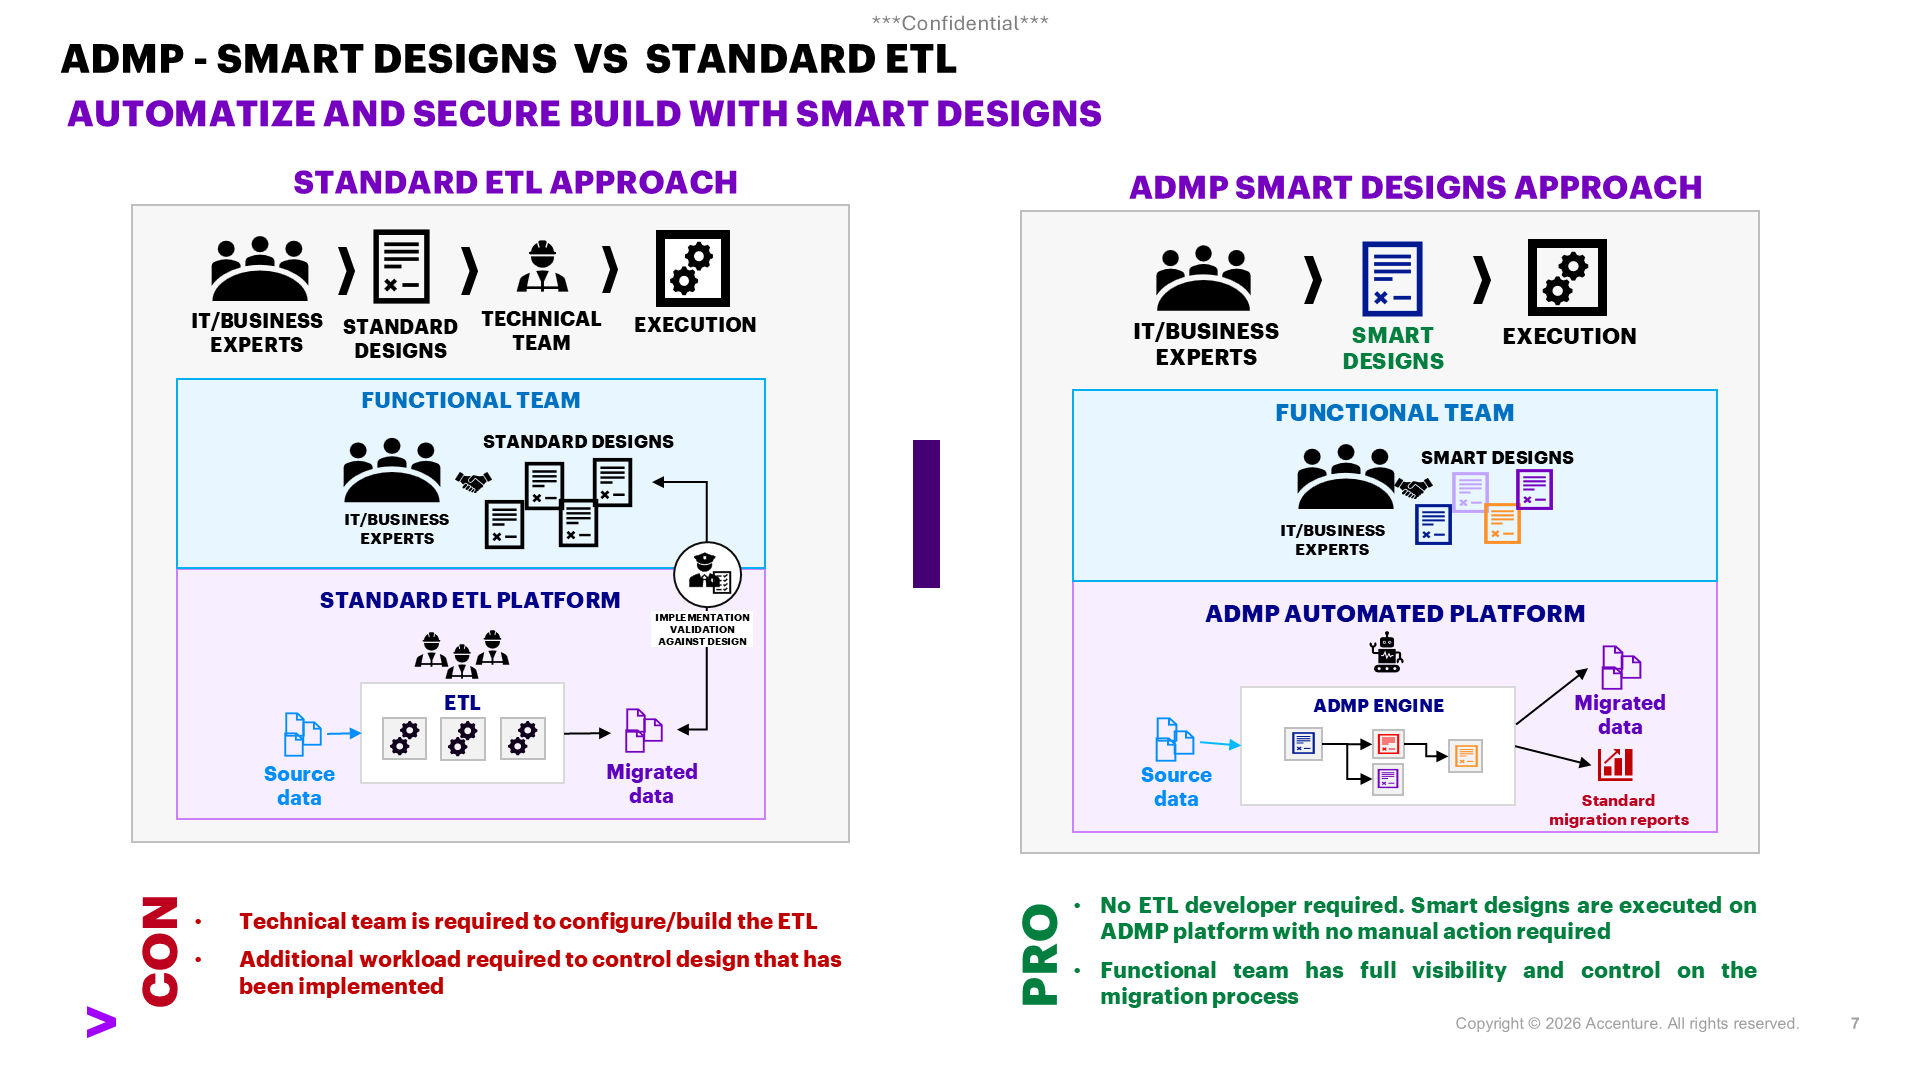
\includegraphics[width=0.85\textwidth]{img/admp_smartdesigns_vs_etl.png}
    \caption{Comparaison visuelle ADMP Smart Designs vs Standard ETL}
    \label{fig:admp-vs-etl}
\end{figure}

La comparaison entre l'approche ADMP Smart Designs et l'approche ETL traditionnelle met en évidence des avantages structurels significatifs, synthétisés dans le Tableau~\ref{tab:admp-vs-etl}.

\begin{table}[H]
\centering
\caption{Comparaison ADMP Smart Designs vs ETL standard}
\label{tab:admp-vs-etl}
\begin{tabularx}{\textwidth}{lXX}
\toprule
\textbf{Domaine} & \textbf{ETL Standard} & \textbf{ADMP Smart Designs} \\
\midrule
Build & Équipe technique requise (Talend, Informatica, BODS) & Aucun développeur ETL requis \\
\addlinespace
Rapports & Développés en supplément de l'ETL & Générés automatiquement depuis les Smart Designs \\
\addlinespace
Scalabilité & Contrainte par l'équipe technique et les outils & Gérée par design, templates hautement distribués \\
\addlinespace
Réutilisabilité & Compétences techniques avancées requises & Personnalisation facile (Word/Excel) \\
\addlinespace
Mises à jour des règles & Mise à jour simultanée des documents \textit{et} de l'ETL & Mise à jour du Smart Design uniquement \\
\addlinespace
Traçabilité & Impossible de valider design vs implémentation & Une seule source de vérité, traçabilité complète \\
\addlinespace
Licence & Coût de licence requis & Aucun coût de licence \\
\bottomrule
\end{tabularx}
\end{table}

% ---------------------------------------------------------------------
\subsubsection{La méthodologie ADMP : notre approche détaillée}
\label{subsubsec:admp-approche}

La méthodologie ADMP structure la migration en quatre phases, chacune impliquant des rôles précis côté client et côté Accenture.

\paragraph{Phase 1 --- Extraction des données.}

\begin{figure}[H]
    \centering
    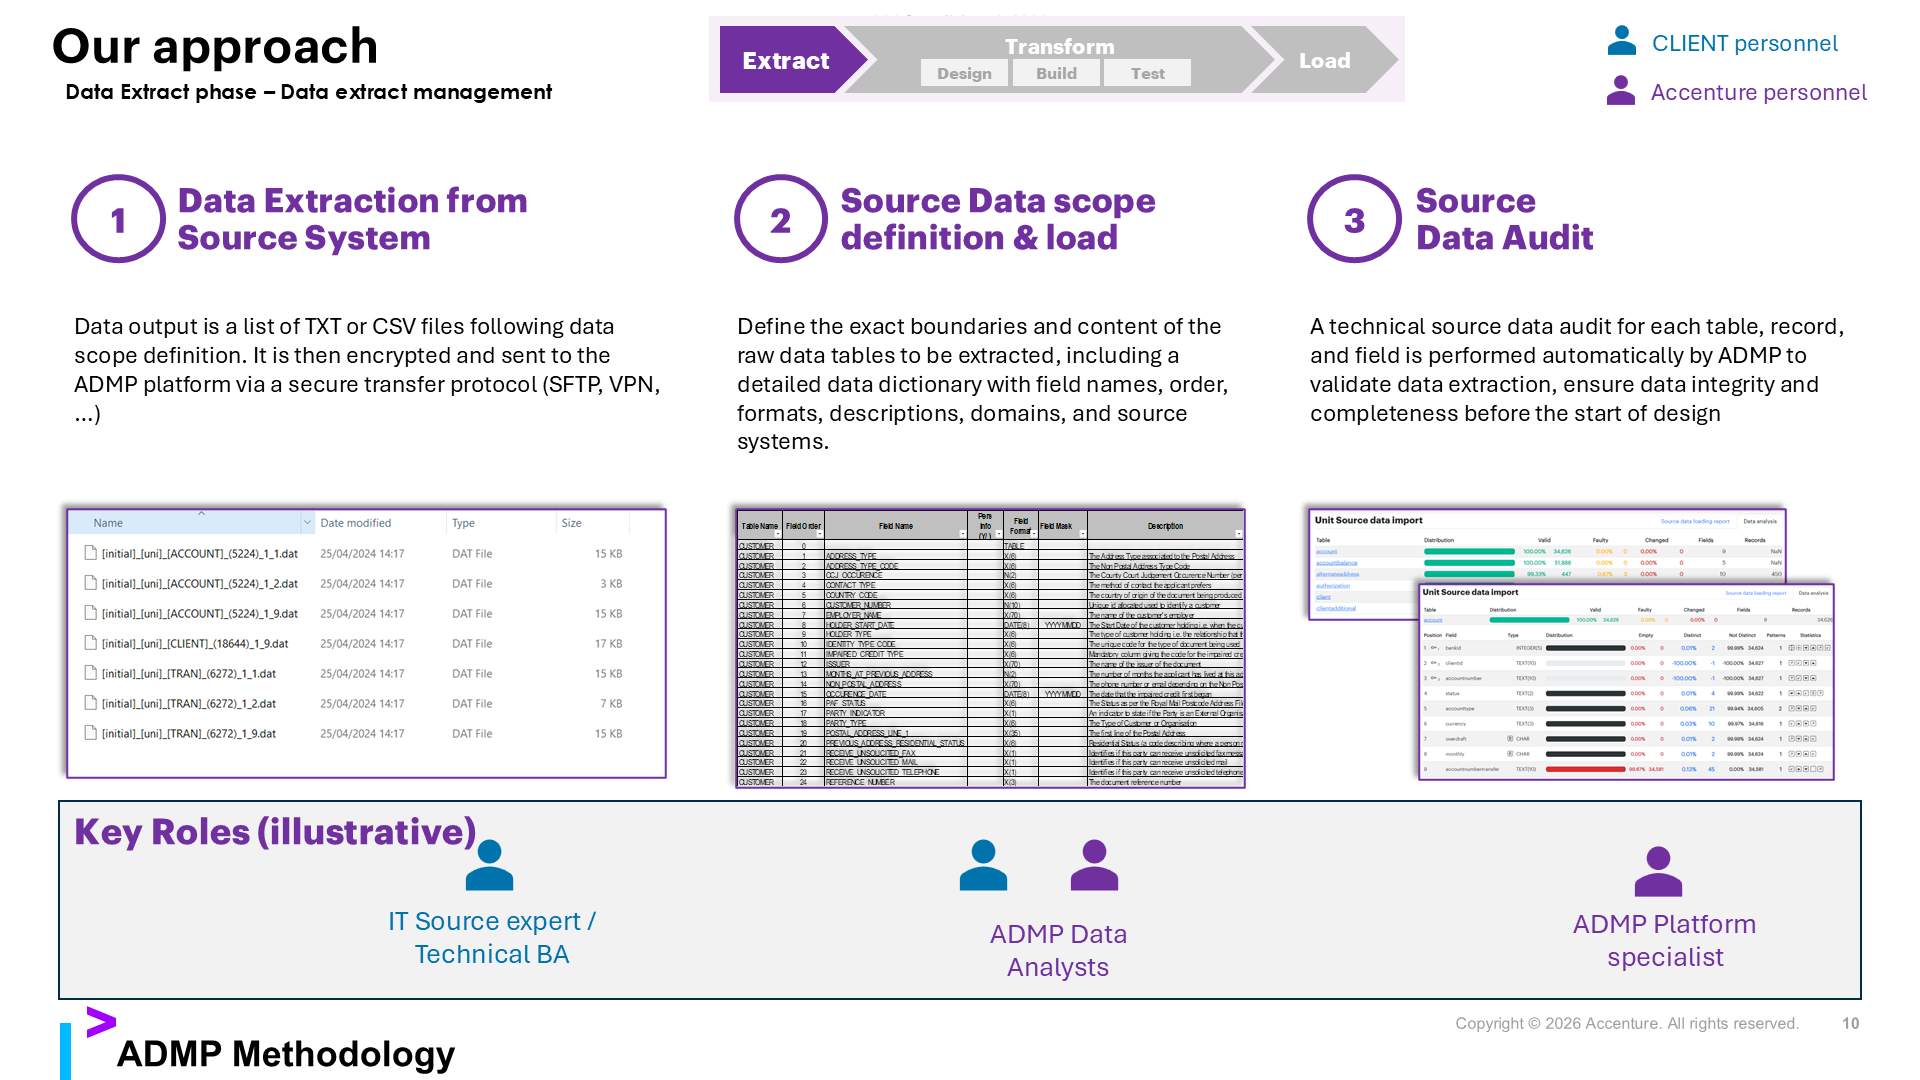
\includegraphics[width=\textwidth]{img/admp_approach_extract.png}
    \caption{Phase d'extraction -- Rôles et activités ADMP}
    \label{fig:admp-extract}
\end{figure}

Cette phase comprend trois étapes : (1) la \textbf{définition du périmètre et chargement} des données source, incluant un dictionnaire de données détaillé (noms de champs, formats, descriptions, domaines et systèmes source) ; (2) l'\textbf{extraction} des données depuis le système source vers des fichiers TXT ou CSV, chiffrés et transmis via SFTP/VPN ; (3) l'\textbf{audit technique automatique} des données source par table, enregistrement et champ.

\paragraph{Phase 2 --- Design (Analyse et Conception détaillée).}

\begin{figure}[H]
    \centering
    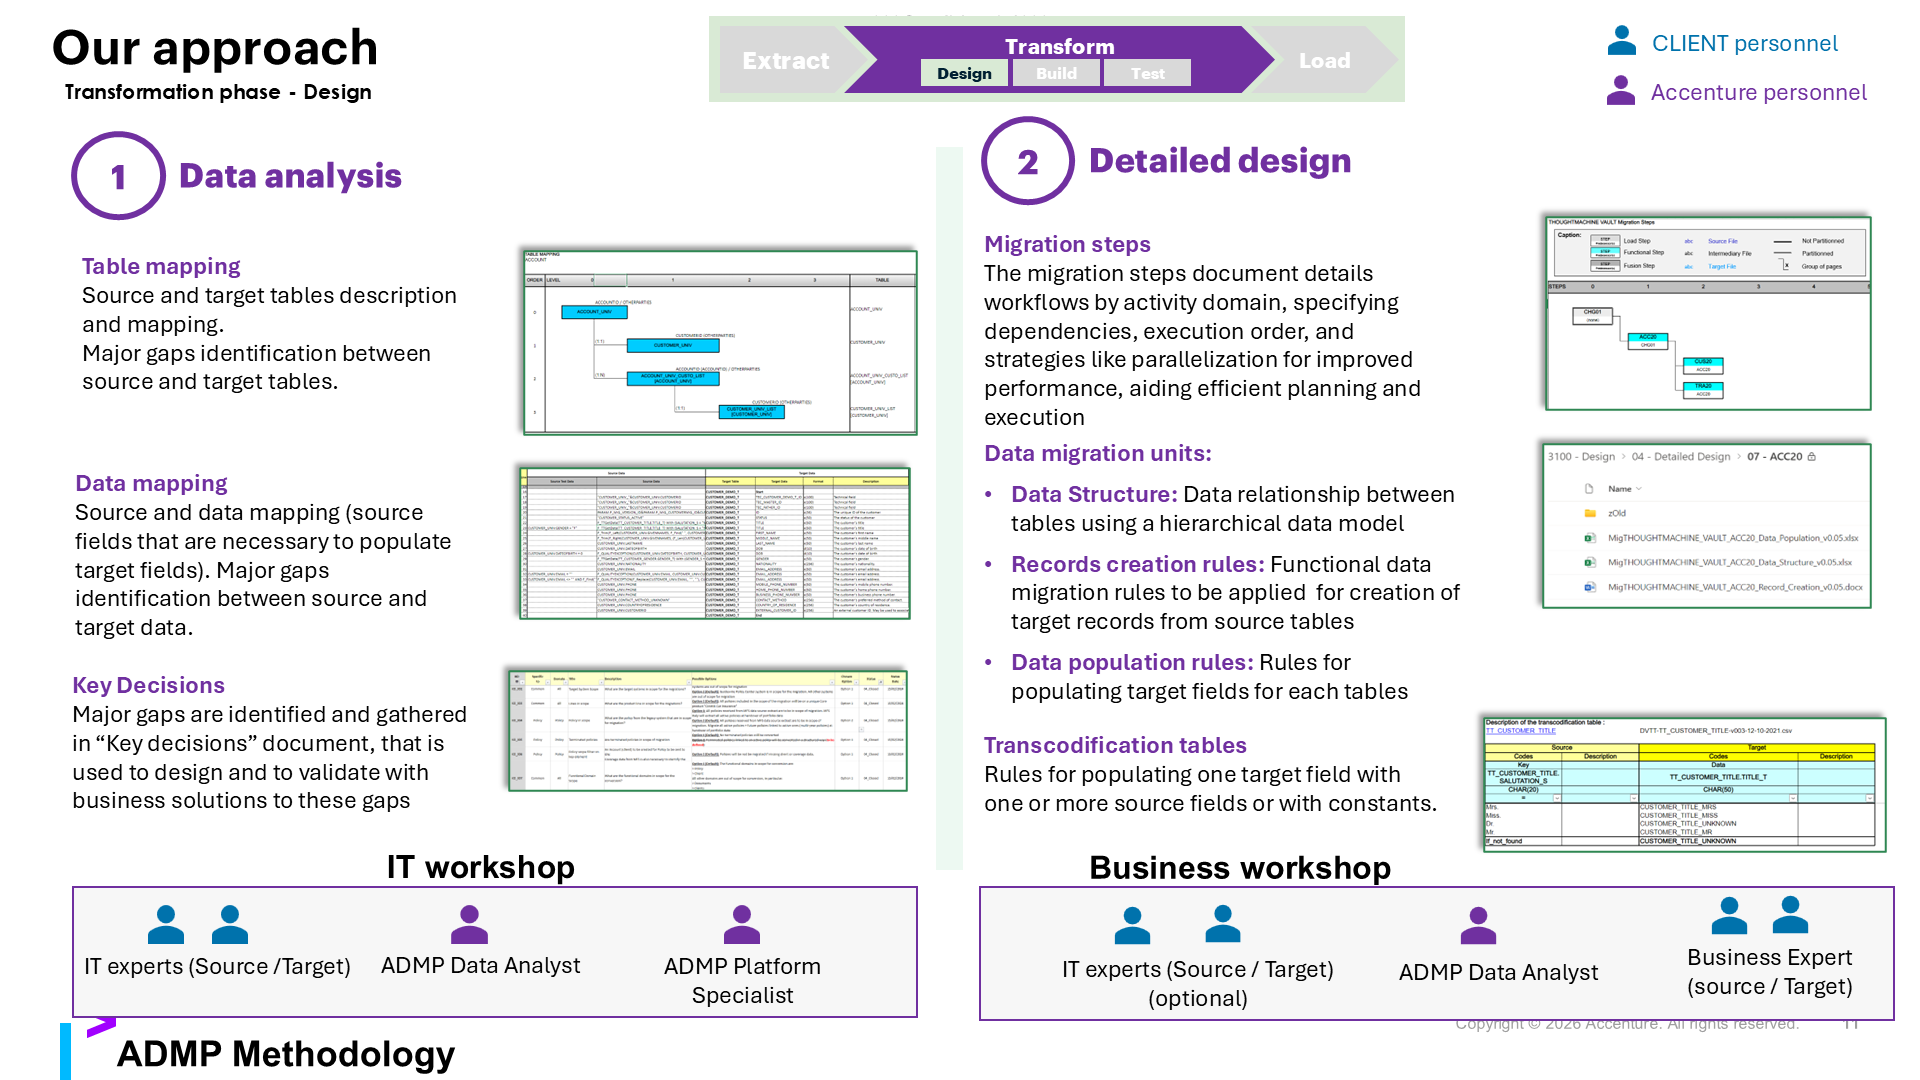
\includegraphics[width=\textwidth]{img/admp_approach_design.png}
    \caption{Phase de design -- Analyse et conception détaillée ADMP}
    \label{fig:admp-design}
\end{figure}

Organisée en deux volets : (1) l'\textbf{analyse de données} (Table Mapping, Data Mapping, Key Decisions pour les écarts majeurs), validée en workshops IT et Business ; (2) la \textbf{conception détaillée} comprenant les Migration Steps (workflows par domaine avec dépendances et stratégies de parallélisation), les Transcodification Tables, et les Data Migration Units (Data Structure, Record Creation, Data Population).

\paragraph{Phase 3 --- Build.}

\begin{figure}[H]
    \centering
    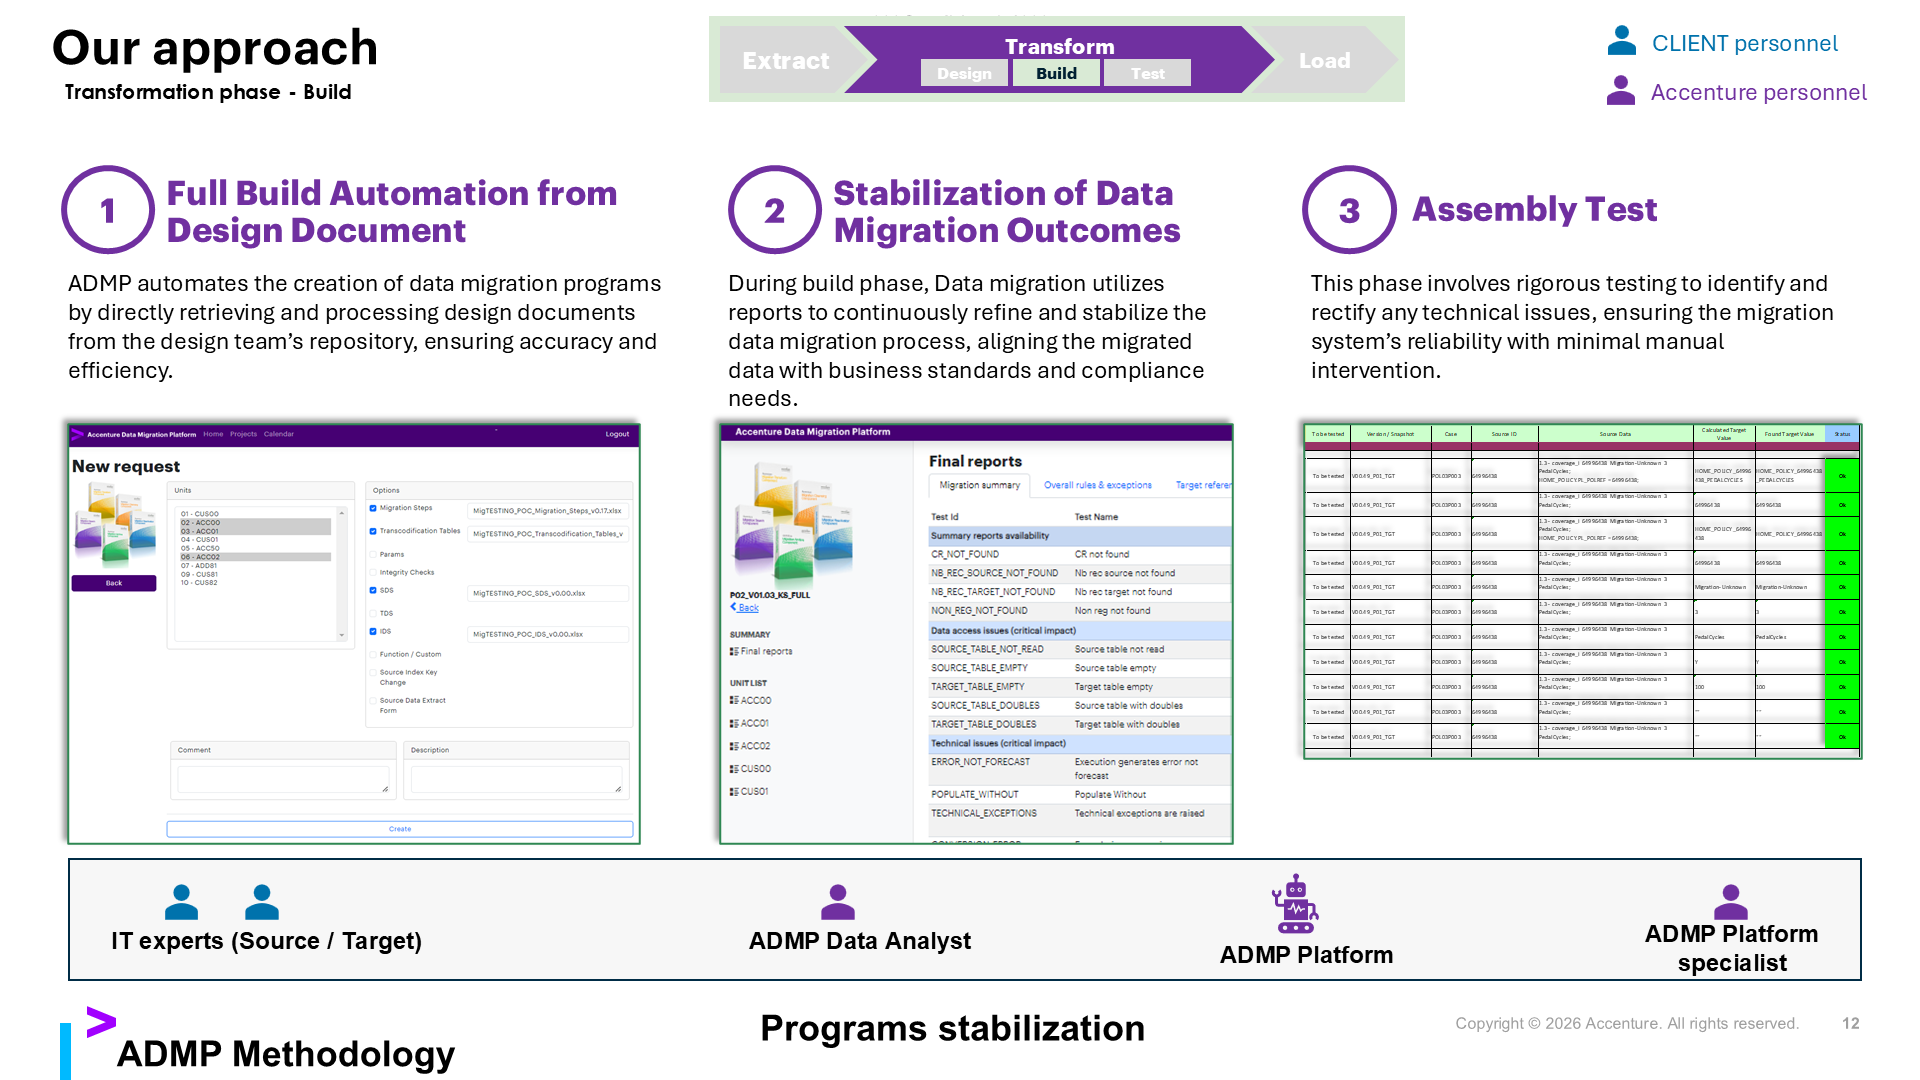
\includegraphics[width=\textwidth]{img/admp_approach_build.png}
    \caption{Phase de build -- Automatisation complète depuis les Smart Designs}
    \label{fig:admp-build}
\end{figure}

ADMP automatise intégralement la création des programmes de migration depuis les documents de design : (1) \textbf{Full Build Automation} -- le moteur récupère et traite directement les documents depuis le dépôt de l'équipe design ; (2) \textbf{Assembly Test} -- tests rigoureux pour identifier et corriger les problèmes techniques avec un minimum d'intervention manuelle ; (3) \textbf{Stabilisation} -- raffinement continu du processus à l'aide des rapports, pour aligner les données migrées avec les standards métier et de conformité.

\paragraph{Phase 4 --- Test et Déploiement.}

\begin{figure}[H]
    \centering
    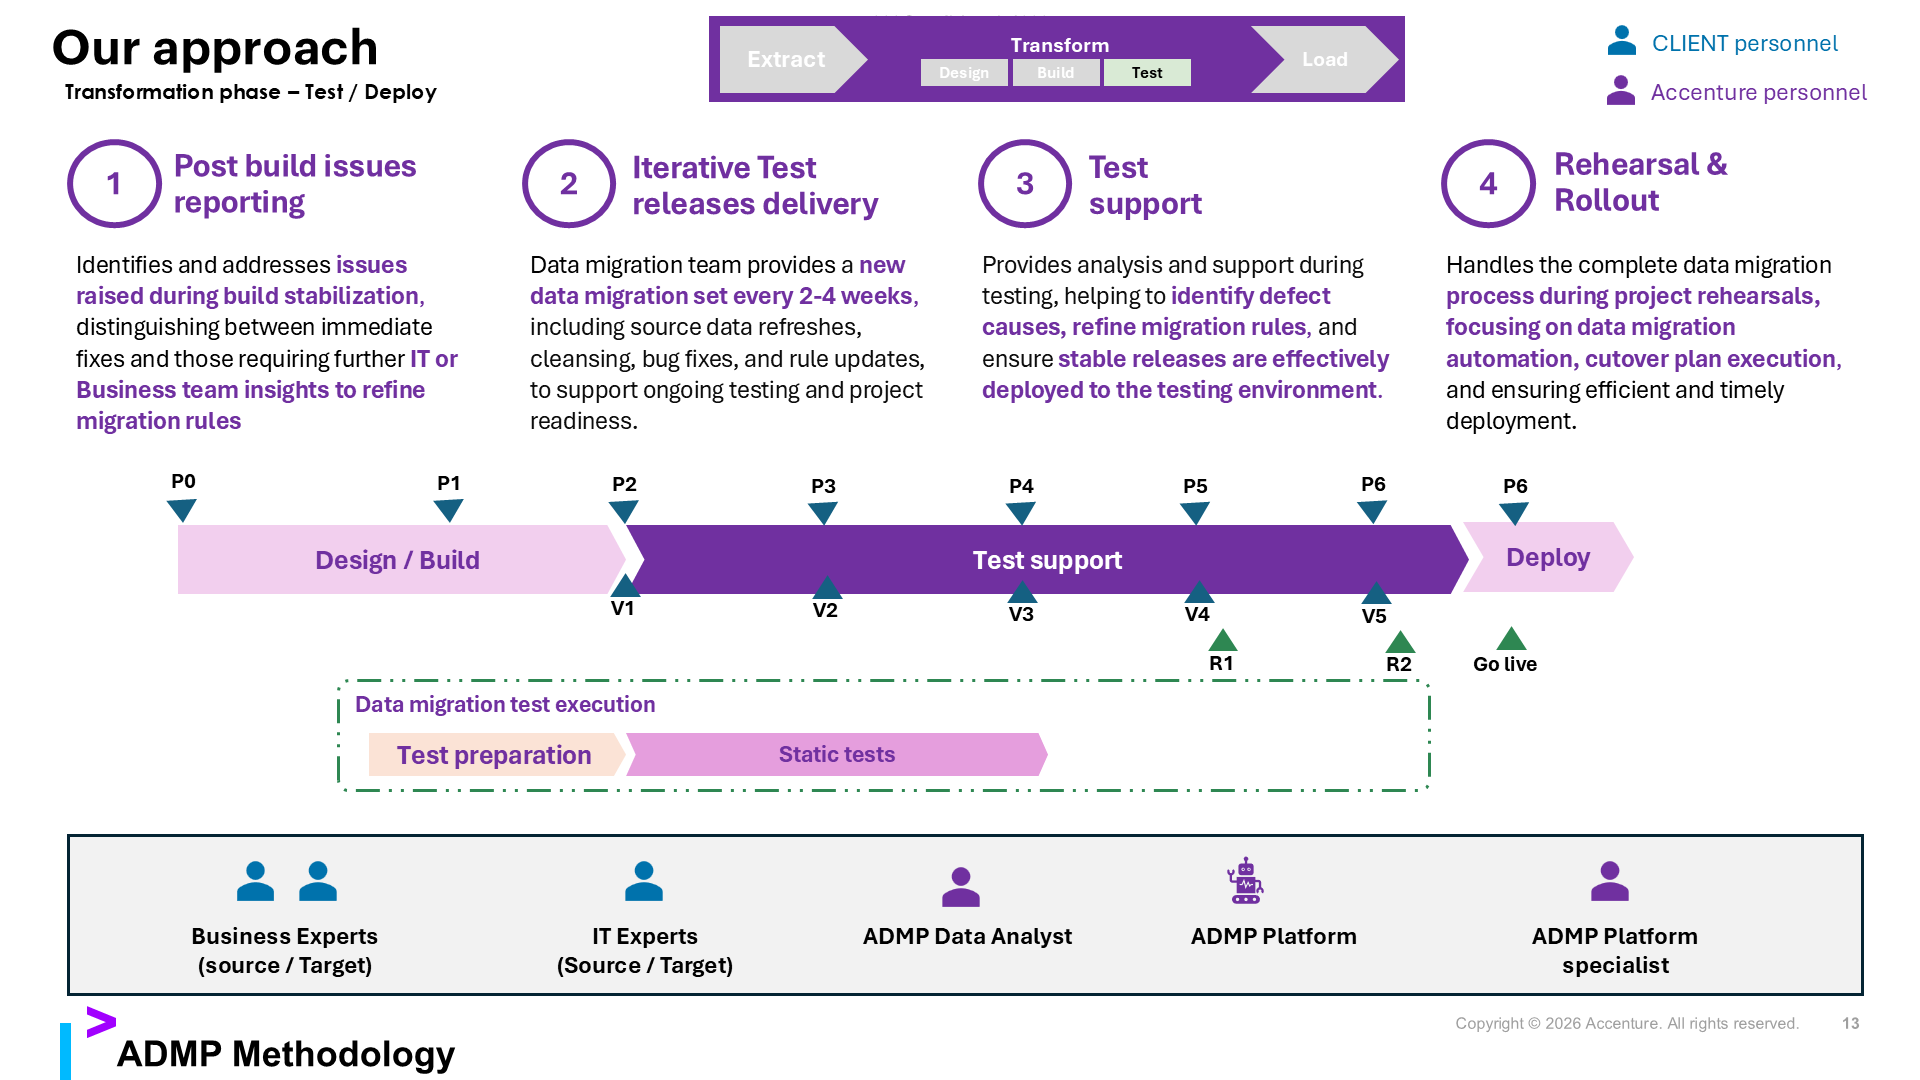
\includegraphics[width=\textwidth]{img/admp_approach_test_deploy.png}
    \caption{Phase de test et déploiement -- Cycle itératif ADMP}
    \label{fig:admp-test-deploy}
\end{figure}

La phase suit un cycle itératif organisé autour de : (1) \textbf{Post-build issues reporting} -- identification des anomalies, distinguant les correctifs immédiats des sujets nécessitant l'input des équipes IT ou Business ; (2) \textbf{Livraisons itératives de releases test} -- une nouvelle version toutes les 2 à 4 semaines (refresh des données source, corrections, mises à jour des règles) ; (3) \textbf{Test support} -- analyse et support lors des tests, identification des causes de défauts et affinement des règles ; (4) \textbf{Rehearsal \& Rollout} -- gestion complète du processus lors des répétitions (\textit{rehearsals}) et exécution du plan de bascule (\textit{cutover}).

% =====================================================================
\subsection{Intelligence artificielle et intégration de données}
\label{subsec:ia-integration}

% ---------------------------------------------------------------------
\subsubsection{LLM et génération de code (GPT, Mistral, fine-tuning, LoRA)}
\label{subsubsec:llm}

Les \textbf{Large Language Models (LLM)} ont révolutionné le domaine de la génération automatique de code et de la compréhension du langage naturel. Des modèles comme GPT-4, Llama 3, Claude et Mistral sont capables de générer du code SQL, Python ou PySpark à partir de spécifications en langage naturel, ouvrant des perspectives considérables pour l'automatisation des processus de migration.

La technique de \textbf{LoRA (Low-Rank Adaptation)}, introduite par Hu et al. (2021), a transformé l'approche du fine-tuning en permettant d'adapter des modèles de plusieurs milliards de paramètres avec une fraction des ressources habituellement nécessaires. LoRA gèle les poids du modèle pré-entraîné et injecte des matrices de rang faible entraînables dans chaque couche, réduisant les paramètres entraînables de \textbf{99\%+} tout en atteignant \textbf{95-98\% de la performance} d'un fine-tuning complet.

Concrètement, le fine-tuning d'un modèle Llama 3.1 70B passe de \textbf{8 GPU A100 pendant 48 heures ($\sim$15 000 \$)} en fine-tuning complet à \textbf{1 GPU A100 pendant 4 heures ($\sim$500 \$)} avec LoRA. Cette démocratisation rend le fine-tuning accessible pour des cas d'usage spécifiques à un domaine, comme la génération de règles de transformation de données.

La variante \textbf{QLoRA} combine LoRA avec une quantification 4-bit, permettant le fine-tuning sur du matériel grand public, une avancée particulièrement pertinente pour les équipes ne disposant pas d'infrastructure GPU dédiée.

\begin{figure}[H]
    \centering
    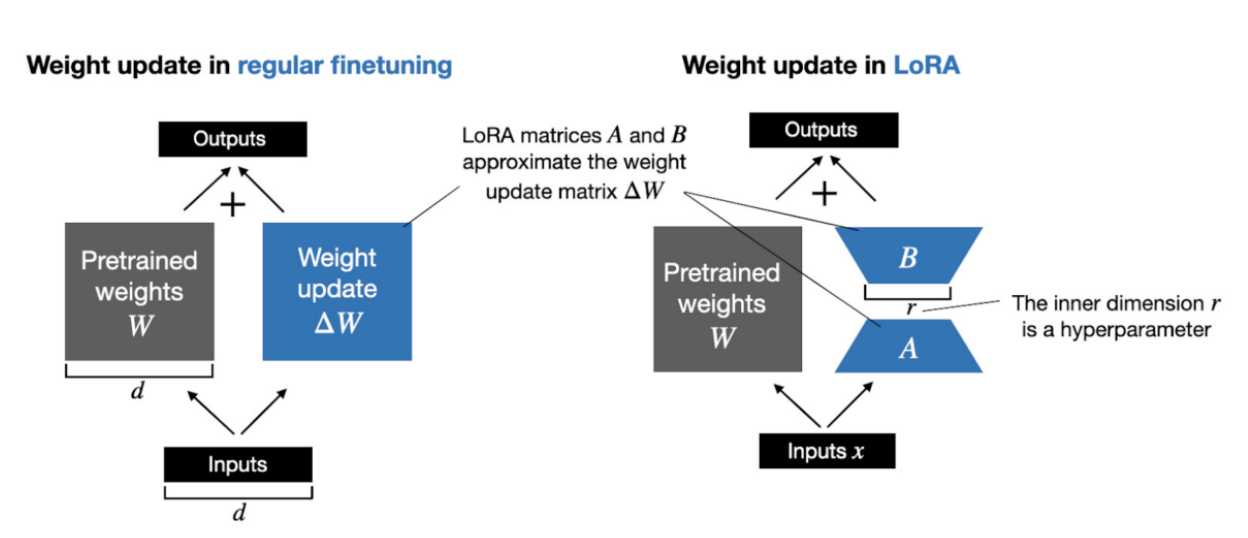
\includegraphics[width=0.8\textwidth]{img/LoRa.png}
    \caption{Principe du fine-tuning avec LoRA (Low-Rank Adaptation)}
    \label{fig:lora}
\end{figure}

% ---------------------------------------------------------------------
\subsubsection{RAG (Retrieval-Augmented Generation)}
\label{subsubsec:rag}

Le \textbf{RAG (Retrieval-Augmented Generation)}, introduit par Lewis et al. (2020), est une architecture qui enrichit les LLM en les couplant avec des sources de connaissances externes au moment de l'inférence. Plutôt que de s'appuyer uniquement sur les connaissances intériorisées lors de l'entraînement, le RAG récupère dynamiquement des passages pertinents depuis une base documentaire et les injecte dans le contexte du modèle pour générer des réponses factuellement ancrées.

L'architecture RAG se décompose en deux composants principaux :

\begin{itemize}[leftmargin=*]
    \item \textbf{Le composant de récupération} : les requêtes sont encodées en vecteurs denses, puis comparées aux vecteurs de documents pré-encodés dans une base vectorielle (FAISS, pgvector, Pinecone). Les passages les plus pertinents sont extraits.
    
    \item \textbf{Le composant de génération} : les documents récupérés sont combinés avec la requête pour produire une réponse contextuelle et précise via le LLM.
\end{itemize}

Microsoft propose une architecture RAG de référence dans Azure Architecture Center, intégrant Azure AI Search, Semantic Kernel et des modèles de langage pour construire des applications d'entreprise robustes.

Dans le contexte de la migration de données, le RAG permet d'exploiter la documentation existante (SDS, TDS, RC, DP) comme base de connaissances pour assister les spécificateurs dans la rédaction de règles, la résolution de questions fonctionnelles, et la validation des designs.

\begin{figure}[H]
    \centering
    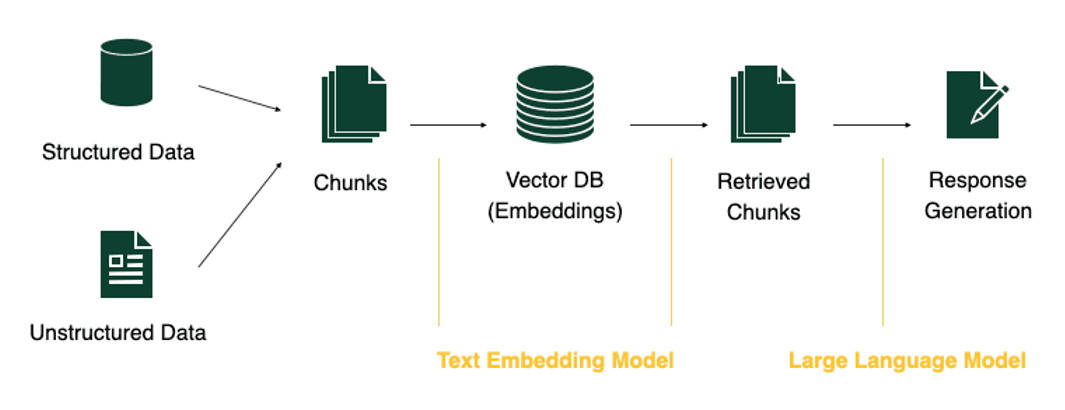
\includegraphics[width=0.9\textwidth]{img/RAG.png}
    \caption{Architecture Retrieval-Augmented Generation (RAG)}
    \label{fig:rag-architecture}
\end{figure}

% ---------------------------------------------------------------------
\subsubsection{Agents IA et automatisation de workflows}
\label{subsubsec:agents-ia}

Les \textbf{agents IA} représentent une évolution majeure par rapport à l'automatisation traditionnelle. Contrairement aux systèmes RPA (\textit{Robotic Process Automation}) qui suivent des scripts prédéfinis, les agents IA combinent perception, raisonnement et action pour accomplir des objectifs de manière autonome.

Leurs caractéristiques distinctives incluent :

\begin{itemize}[leftmargin=*]
    \item \textbf{Autonomie} : fonctionnement indépendant sans supervision constante.
    \item \textbf{Conscience contextuelle} : compréhension des scénarios métier nuancés.
    \item \textbf{Raisonnement multi-étapes} : décomposition de tâches complexes en sous-tâches exécutables.
    \item \textbf{Auto-correction} : identification et rectification des erreurs en cours d'exécution.
    \item \textbf{Intégration d'outils} : connexion transparente avec APIs, bases de données et systèmes d'entreprise.
\end{itemize}

Le marché mondial des agents IA est estimé à \textbf{5,1 milliards USD en 2024}, avec une projection à \textbf{47,1 milliards USD d'ici 2030} (CAGR de 44,8\%). Toutefois, selon Gartner (2025), moins de \textbf{5\% des applications d'entreprise intègrent de véritables agents IA} à ce stade, la majorité n'utilisant que des assistants basiques.

% ---------------------------------------------------------------------
\subsubsection{Applications de l'IA dans la migration de données}
\label{subsubsec:ia-migration}

L'application de l'IA au domaine spécifique de la migration de données est un champ émergent mais prometteur, avec cinq cas d'usage à fort impact identifiés par Blackburn (2025) :

\begin{itemize}[leftmargin=*]
    \item \textbf{Mapping automatique de schémas} : les modèles ML analysent la structure, le contenu et les métadonnées des sources pour suggérer des correspondances source-cible, réduisant le temps de mapping de \textbf{30-60\%}.
    
    \item \textbf{Évaluation et nettoyage de la qualité} : les LLM détectent les anomalies que les règles statiques ne capturent pas, et peuvent suggérer des actions de nettoyage automatiques.
    
    \item \textbf{Génération de données synthétiques de test} : les modèles génératifs produisent des jeux de test réalistes préservant les propriétés statistiques sans exposer de données réelles.
    
    \item \textbf{Planification intelligente de la migration} : le reinforcement learning optimise l'ordonnancement des lots de migration en fonction des dépendances et des contraintes de fenêtre.
    
    \item \textbf{Monitoring et détection d'anomalies en production} : des pipelines de détection identifient les écarts en temps réel et accélèrent le triage des erreurs.
\end{itemize}

La plateforme \textbf{MAiGRATE} de Compliance Group illustre cette tendance : elle combine IA, ML et LLM pour automatiser l'ingestion, la transformation, le mapping de champs, la déduplication, la détection d'anomalies et la validation, avec un apprentissage continu améliorant la précision à chaque cycle de migration.

% =====================================================================
\subsection{Limites de l'existant et opportunités}
\label{subsec:limites-opportunites}

% ---------------------------------------------------------------------
\subsubsection{Limites des outils de design actuels}
\label{subsubsec:limites-design}

Les Design Tools actuels d'ADMP reposent sur des \textbf{plugins VBA intégrés à Word et Excel}. Si cette approche a l'avantage d'utiliser des outils familiers aux équipes fonctionnelles, elle présente des limitations de plus en plus critiques :

\begin{itemize}[leftmargin=*]
    \item \textbf{Technologie vieillissante} : VBA est un langage de macro datant des années 1990, dont le support et l'évolutivité sont limités.
    \item \textbf{Pas de collaboration en temps réel} : contrairement aux outils web modernes, les documents Word/Excel ne permettent pas l'édition simultanée avec traçabilité fine.
    \item \textbf{Intégration IA impossible} : l'architecture VBA ne permet pas d'intégrer nativement des appels à des API d'IA (OpenAI, Bedrock) pour assister la rédaction.
    \item \textbf{Maintenance complexe} : les macros VBA sont fragiles, sensibles aux versions d'Office, et difficiles à déboguer.
\end{itemize}

% ---------------------------------------------------------------------
\subsubsection{Rédaction manuelle des spécifications}
\label{subsubsec:redaction-manuelle}

La rédaction des spécifications de migration (RC, DP, DS, TT) reste un processus \textbf{largement manuel et chronophage}. Chaque document nécessite une compréhension approfondie du modèle source, du modèle cible, et des règles métier spécifiques. Comme le souligne la présentation d'évolution ADMP, l'un des objectifs stratégiques de la modernisation est de \og~\textit{Optimize and accelerate the time needed to write specifications}~\fg{} et de \og~\textit{Create a true wizard for specifiers and reduce the overall burden}~\fg{}.

Le rapport PFE de Abbad el andaloussi, Larbi estime que l'automatisation de la génération des livrables de migration permettrait une \textbf{réduction de 50 à 60\% du temps} nécessaire à leur production, tout en minimisant les risques d'erreurs humaines.

% ---------------------------------------------------------------------
\subsubsection{Absence d'IA dans le processus de migration}
\label{subsubsec:absence-ia}

Malgré les avancées considérables de l'IA dans d'autres domaines de l'IT, le processus de migration ADMP reste \textbf{dépourvu d'intelligence artificielle}. Aucun module IA n'assiste actuellement les spécificateurs dans la rédaction des règles, la détection des incohérences, ou la validation automatique des designs. Cette absence représente une opportunité majeure d'amélioration.

% ---------------------------------------------------------------------
\subsubsection{Dépendance à l'expertise humaine}
\label{subsubsec:dependance-expertise}

La qualité de la migration repose fortement sur l'expertise individuelle des Data Analysts. L'\textbf{onboarding} de nouveaux membres nécessite une formation intensive (la CIDS dure \textbf{2 semaines (80 heures)}) et l'acquisition de la maturité opérationnelle prend plusieurs mois supplémentaires. Cette dépendance crée un risque de perte de connaissances (\textit{knowledge drain}) lors des rotations d'équipe et limite la scalabilité des opérations.

% =====================================================================
\subsection{Synthèse et positionnement de la contribution}
\label{subsec:synthese-positionnement}

% ---------------------------------------------------------------------
\subsubsection{Tableau de synthèse des gaps identifiés}
\label{subsubsec:gaps}

Le Tableau~\ref{tab:gaps-synthesis} synthétise les principaux gaps identifiés et les opportunités associées.

\begin{table}[H]
\centering
\caption{Synthèse des gaps identifiés et opportunités}
\label{tab:gaps-synthesis}
\begin{tabularx}{\textwidth}{XXX}
\toprule
\textbf{Gap identifié} & \textbf{Impact} & \textbf{Opportunité} \\
\midrule
Outils de design VBA obsolètes & Pas de collaboration, pas d'IA & → ADMP Studio (outil web moderne) \\
\addlinespace
Rédaction manuelle des spécifications & Chronophage, risque d'erreur & → ADMP AI Engine (génération assistée) \\
\addlinespace
Absence d'IA dans le processus & Aucune assistance intelligente & → Intégration LLM + RAG \\
\addlinespace
Dépendance à l'expertise humaine & Onboarding long, scalabilité limitée & → Assistant IA pour spécificateurs \\
\addlinespace
Pas de génération automatique de code & Build manuel des programmes & → Bundle Databricks (notre contribution) \\
\bottomrule
\end{tabularx}
\end{table}

% ---------------------------------------------------------------------
\subsubsection{Positionnement du PFE}
\label{subsubsec:positionnement-pfe}

L'analyse de l'état de l'art révèle que la plateforme ADMP, malgré sa maturité et ses avantages concurrentiels significatifs, se trouve à un tournant stratégique. Les outils existants ont prouvé leur efficacité pendant plus de 25 ans, mais l'absence d'intelligence artificielle dans le processus constitue désormais un frein à l'innovation et à la compétitivité.

Le programme d'évolution d'ADMP, articulé autour de l'\textbf{ADMP AI Engine}, de l'\textbf{ADMP Studio} et de l'amélioration des outils de design, vise à combler ces gaps.

Notre contribution, le \textbf{développement du module de génération du bundle Databricks}, s'inscrit précisément dans cet axe d'industrialisation. Ce module vise à automatiser la création des artefacts de migration en s'appuyant sur des technologies de traitement distribué (Apache Spark / Databricks) et d'intelligence artificielle générative, transformant ainsi les Smart Designs en programmes exécutables sur des infrastructures cloud modernes.

Ce positionnement se situe à l'intersection de trois tendances identifiées dans l'état de l'art : l'\textbf{automatisation du cycle Design-Build} (section~\ref{subsec:admp-actuel}), l'\textbf{application de l'IA à la migration} (section~\ref{subsec:ia-integration}), et le besoin de \textbf{modernisation des outils} (section~\ref{subsec:limites-opportunites}). Le chapitre suivant présentera le cadre méthodologique et organisationnel dans lequel ce travail a été réalisé.